\documentclass[11pt,a4paper,english,draft]{article}
\usepackage[english]{babel} % Using babel for hyphenation
\usepackage{lmodern} % Changing the font
\usepackage[utf8]{inputenc}
\usepackage[T1]{fontenc}

%\usepackage[moderate]{savetrees} % [subtle/moderate/extreme] really compact writing
\usepackage{tcolorbox}
\tcbuselibrary{hooks}
\usepackage[parfill]{parskip} % Removes indents
\usepackage{amsmath} % Environment, symbols etc...
\usepackage{amssymb}
\usepackage{float} % Fixing figure locations
\usepackage{multirow} % For nice tables
%\usepackage{wasysym} % Astrological symbols
\usepackage{graphicx} % For pictures etc...
\usepackage{enumitem} % Points/lists
\usepackage{physics} % Typesetting of mathematical physics examples: 
                     % \bra{}, \ket{}, expval{}
\usepackage{url}

\definecolor{red}{RGB}{255,10,10}

% To include code(-snippets) with æøå
\usepackage{listings}
\lstset{
language=c++,
showspaces=false,
showstringspaces=false,
frame=l,
}

\tolerance = 5000 % Bedre tekst
\hbadness = \tolerance
\pretolerance = 2000

\numberwithin{equation}{section}

\newcommand{\conj}[1]{#1^*}
\newcommand{\ve}[1]{\mathbf{#1}} % Vektorer i bold
\let\oldhat\hat
\renewcommand{\hat}[1]{\oldhat{#1}}
\newcommand{\trans}[1]{#1^\top}
\newcommand{\herm}[1]{#1^\dagger}
%\renewcommand{\thefootnote}{\fnsymbol{footnote}} % Gir fotnote-symboler
\newcommand{\Real}{\mathbb{R}}
\newcommand{\bigO}[1]{\mathcal{O}\left( #1 \right)}

\newcommand{\spac}{\hspace{5mm}}



\newcounter{algcounter}
\renewcommand{\thealgcounter}{\Roman{algcounter}}

\newenvironment{algorithm}{%
\refstepcounter{algcounter}
\begin{tcolorbox}
\centerline{Algorithm \thealgcounter}\vspace{2mm}
}
{\end{tcolorbox}}

\newcommand{\figurewidth}{.85\textwidth}

\title{FYS3150/4150\\Computational Physics\\Project 2}
\author{Magnus Ulimoen\\Krister Stræte Karlsen}
\date{\today}

\begin{document}
\tcbset{before app=\parfillskip0pt}
\maketitle

\section{Introduction}

In this project the Schrödinger's equation for two electrons in a
three-dimensional harmonic oscillator well will be solved numerically. 
Both computational and physical aspects of the problem will be discussed 
throughout the report. 


\section{Method}

\subsection{Schrödinger's equation}


\subsubsection{Time-independent Schrödinger's equation}
From quantum mechanics we have Schrödinger's equation on the form
\begin{equation}
\hat{H} \ket{\Psi} = i\hbar \frac{\partial }{\partial t} \ket{\Psi}
\label{eq:Schrödinger}
\end{equation}
If the Hamiltonian $\hat{H}$ is independent of time this is separable,
and the left side of \eqref{eq:Schrödinger} is taken as E, and we get the
time-independent Schrödinger equation;
\begin{equation}
 \hat{H}\ket{\Psi} = E\ket{\Psi}
\end{equation}
For a single electron the Hamiltonian has the form 
\begin{equation}
\hat{H} = \frac{\hat{p}^2}{2m} + V(\ve{r})
\end{equation}
Or if written in the function basis,
\begin{equation}
\hat{H} = -\frac{\hbar^2}{2m}\nabla^2 + V(\ve{r})
\label{eq:Hamiltonian}
\end{equation}



\subsubsection{Spherical harmonics}
Writing out \eqref{eq:Hamiltonian} in spherical coordinates we end up
with the equation
\begin{gather}
\nonumber \hat{H} = \\
-\frac{\hbar^2}{2m}\left(\frac{1}{r^2}\frac{\partial}{\partial r}
\left( r^2\frac{\partial }{\partial r}\right)
+ \frac{1}{r^2}\left[ \frac{1}{\sin\theta}\frac{\partial}{\partial \theta}
\left( \sin\theta \frac{\partial}{\partial \theta}\right)
+ \frac{1}{\sin^2\theta}\frac{\partial^2}{\partial \phi^2}
\right]\right) + V(r,\theta,\phi)
\end{gather}
If $V$ is spherically symmetrical, the solution is separable into
$\Psi = R(r)Y_l^m(\theta, \phi)$ where $Y_l^m$ is the associated Laguerre
polynomials. The part in the square brackets is an eigenfunction of 
$Y_l^m$, with eigenvalue $-l(l+1)$. 


\subsubsection{Radial equation}

The radial part of the Schrödinger's equation now reads:
\begin{gather}
  -\frac{\hbar^2}{2 m} \left ( \frac{1}{r^2} \frac{d}{dr} r^2
  \frac{d}{dr} - \frac{l (l + 1)}{r^2} \right )R(r) 
     + V(r) R(r) = E R(r)
\label{eq:radial}
\end{gather}
The $l$ quantum number tends to ''throw'' the radial part outwards,
and works as a centrifugal barrier.

\subsection{Harmonic oscillator}
In our case $V(r)$ is the harmonic oscillator potential 
$V = \frac{1}{2}k r^2$ with
$k=m\omega^2$. 

We make the substitution $R(r) = (1/r) u(r)$ in the radial
equation and obtain
\begin{gather}
  -\frac{\hbar^2}{2 m} \frac{d^2}{dr^2} u(r) 
       + \left ( V(r) + \frac{l (l + 1)}{r^2}\frac{\hbar^2}{2 m}
                                    \right ) u(r)  = E u(r) .
\end{gather}
The boundary conditions are $u(0)=0$ and $u(\infty)=0$ to avoid
an unnormalizable wave function.

Introducing the dimensionless variable $\rho = (1/\alpha) r$
where $\alpha$ is a constant with dimension length we get
\begin{gather}
  -\frac{\hbar^2}{2 m \alpha^2} \frac{d^2}{d\rho^2} u(\rho) 
       + \left ( V(\rho) + \frac{l (l + 1)}{\rho^2}
         \frac{\hbar^2}{2 m\alpha^2} \right ) u(\rho)  = E u(\rho) .
\end{gather}
In this project we will only study the situation $l=0$.
Inserting $V(\rho) = (1/2) k \alpha^2\rho^2$ we end up with
\begin{gather}
  -\frac{\hbar^2}{2 m \alpha^2} \frac{d^2}{d\rho^2} u(\rho) 
       + \frac{k}{2} \alpha^2\rho^2u(\rho)  = E u(\rho) .
\end{gather}
Multiplying with $2m\alpha^2/\hbar^2$ on both sides to obtain
\begin{gather}
  -\frac{d^2}{d\rho^2} u(\rho) 
       + \frac{mk}{\hbar^2} \alpha^4\rho^2u(\rho) 
       = \frac{2m\alpha^2}{\hbar^2}E u(\rho) .
\end{gather}
The constant $\alpha$ can now be fixed such that
\begin{gather}
\frac{mk}{\hbar^2} \alpha^4 = 1,
\end{gather}
and the constant is now
\begin{gather}
\alpha = \left(\frac{\hbar^2}{mk}\right)^{1/4}
\end{gather}
Defining 
\begin{gather}
\lambda = \frac{2m\alpha^2}{\hbar^2}E,
\end{gather}
we can rewrite Schrödinger's equation as
\begin{equation}
  -\frac{d^2}{d\rho^2} u(\rho) + \rho^2u(\rho)  = \lambda u(\rho) .
\end{equation}

This equation can now be discretized and solved as a linear system 
using for example Jacobi's algorithm for eigenvalues. 

\subsubsection{Eigenvalues of the harmonic oscillator}
The eigenvalues of \eqref{eq:radial} can be found analytically,
and are the energies
\begin{gather}
E_{nl}=  \hbar \omega \left(2n+l+\frac{3}{2}\right),
\end{gather}
where $n$ and $l$ are quantum numbers, with $n = 0, 1, 2, \dots$ and
$l = 0, 1, 2,  \dots $.
 
 \subsubsection{Two electrons in harmonic oscillator}
If two electrons are put in the same potential a respulse Coulomb 
interaction will emerge between them. If we use a relative coordinate
and a COM coordinate, it can be shown that Schrödinger's equation
reduces to
\begin{gather}
 -\frac{d^2}{d\rho^2} \psi(\rho) + \omega_r^2\rho^2\psi(\rho) 
 +\frac{1}{\rho} = \lambda \psi(\rho)
\end{gather}
with $\omega_r$ reflecting the strength of the potential. 

 
 
 
\subsection{Discretization}

Using a standard center approximation for the second derivative:$u$
\begin{equation}
    u''=\frac{u(\rho+h) -2u(\rho) +u(\rho-h)}{h^2} +O(h^2),
    \label{eq:diffoperation}
\end{equation} 
where $h$ is our step length.

For a finite value of $\rho_{\mathrm{max}}$, we can define 
\begin{gather}
  h=\frac{\rho_{\mathrm{max}}-\rho_{\mathrm{min}} }{n_{\mathrm{step}}}.
\end{gather}
and 
\begin{gather}
    \rho_i= \rho_{\mathrm{min}} + ih, \hspace{1cm} i=0,1,2,\dots ,
    n_{\mathrm{step}}
\end{gather}
Then rewrite the Schrödinger equation for $\rho_i$ as
\begin{gather}
-\frac{u(\rho_i+h) -2u(\rho_i) +u(\rho_i-h)}{h^2}+\rho_i^2u(\rho_i) 
= \lambda u(\rho_i)
\end{gather}
where $V_i=\rho_i^2$ is the harmonic oscillator potential.

Defining 
\begin{gather}
   d_i=\frac{2}{h^2}+V_i, \hspace{0.5cm } e_i=-\frac{1}{h^2}.
\end{gather}
the Schrödinger equation takes the following form
\begin{gather}
d_iu_i+e_{i-1}u_{i-1}+e_{i+1}u_{i+1}  = \lambda u_i,
\end{gather}
where $u_i$ is unknown. We can write the 
latter equation as a matrix eigenvalue problem 
\begin{equation}
\begin{pmatrix} d_1 & e_1 & 0   & 0    & \dots  &0     & 0 \\
                e_1 & d_2 & e_2 & 0    & \dots  &0     &0 \\
                0   & e_2 & d_3 & e_3  &0       &\dots & 0\\
        \dots  & \dots & \dots & \ddots  &\ddots      &\dots & \dots\\
 0   & \dots & \dots & \dots  &\dots  &d_{n_{\mathrm{step}}-2} & e_{n_{\mathrm{step}}-1}\\
 0   & \dots & \dots & \dots  &\dots       &e_{n_{\mathrm{step}}-1} & d_{n_{\mathrm{step}}-1}
             \end{pmatrix}
\begin{pmatrix} u_{1} \\
      u_{2} \\
      \dots\\ \dots\\ \dots\\
      u_{n_{\mathrm{step}}-1}
\end{pmatrix} 
= \lambda \begin{pmatrix} u_{1} \\
                          u_{2} \\
                          \dots\\ \dots\\ \dots\\
                          u_{n_{\mathrm{step}}-1}
             \end{pmatrix} 
      \label{eq:sematrix}
\end{equation} 

Some care has to be taken when the limits are selected. Our 
approach har linear spacing between points, and an upper limit 
of $\rho$ must be chosen. Care has to be taken to make sure the 
solution does not depend upon this selection.

We will now move on the see how we can solve this eivenvalue problem using Jacobi's algorithm. 

\subsection{Jacobi's eigenvalue algorithm}

To obtain the eigenvalues of our matrix we are going to apply similarity transformations so that
\begin{align*}
S_N^T S_{N-1}^T .. S_1^T A S_1 .. S_{N_1} S_{N} = D
\end{align*}
using an orthogonal transformation matrix on the form:
\begin{align*}
\begin{pmatrix} 1 & 0 & \dots   & \dots    & 0     \\
                0 & 1 & 0 & \dots    & 0   \\
                \vdots & 0 & cos(\theta) & \dots  & sin(\theta)        \\
        \vdots  & \dots & \dots & \ddots   &\dots \\
 0   & \dots & -sin(\theta) & \dots  & cos(\theta)  
             \end{pmatrix}
\end{align*}

To make this process effective we hunt down the largest non-diagonal element, say $a_{kl}$, and choose the angle of rotation, $\theta$, so that the $kl$-element of the transformed matrix becomes zero. That means solving
\begin{align*}
(a_{kk}-a_{ll})cos(\theta)sin(\theta)+a_{kl}(cos^2 (\theta) - sin^2 (\theta)) = 0
\end{align*}

Defining the quantities $\tan\theta = t= s/c$, with $s=\sin\theta$ and $c=\cos\theta$ and
\begin{gather}\cot 2\theta=\tau = \frac{a_{ll}-a_{kk}}{2a_{kl}}.
\end{gather}

We can then define the angle $\theta$ so that the non-diagonal matrix elements of the transformed matrix 
 become non-zero and
we obtain the quadratic equation (using $\cot 2\theta=1/2(\cot \theta-\tan\theta)$
\begin{gather}
t^2+2\tau t-1= 0,
\end{gather}
resulting in 
\begin{gather}
  t = -\tau \pm \sqrt{1+\tau^2},
\end{gather}

Here a clever choice of roots must be made. For for a well trained computational physicist this equation should be a red warning sign of loss of numerical precision. To avoid subtraction of to almost equal numbers the following choice should be made:

\begin{align*}
t=  -\tau + \sqrt{1+\tau^2}, \quad   0  \geq \tau \\
t=  -\tau - \sqrt{1+\tau^2}, \quad   \tau <  0
\end{align*}

From the equations above we obtain the following relation for $c$ and $t$
\begin{gather}
   c = \frac{1}{\sqrt{1+t^2}}.
\end{gather}
Knowing that $t \in [0,1]$ we put restrictions such that $c \in [\frac{1}{\sqrt{2}}, 1]$ which focres $\theta$ to be in the interval $[- \frac{\pi}{4},\frac{\pi}{4}]$.  

Choosing the smaller $t$ makes $c$ the larger and minimizes 
\begin{gather}
||{\bf B}-{\bf A}||_F^2=4(1-c)\sum_{i=1,i\ne k,l}^n(a_{ik}^2+a_{il}^2) +\frac{2a_{kl}^2}{c^2}.
\end{gather}




\subsubsection{Implementation}

The Jacobi algorithm takes the form
\begin{algorithm}
\label{alg:jacobi}
Find the largest element, $a_{kl}$, in $A$ \\
Compute $\tau:$
\begin{gather*}
  \tau = \frac{a_{ll}-a_{kk}}{2a_{kl}}
\end{gather*}
Compute t according to: 
\begin{gather*}
t=  -\tau + \sqrt{1+\tau^2}, \quad   0  \geq \tau \\
t=  -\tau - \sqrt{1+\tau^2}, \quad   \tau <  0
\end{gather*}
Set
\begin{gather*}
c= \frac{1}{\sqrt{1+t^2}}, \quad s= ct
\end{gather*}
Compute the new matrix elements:
\begin{align*}
 b_{kl} &= a_{kl}, \quad k,l \neq i,j \\
 b_{ik} &= b_{ki} = ca_{ik}-sa_{jk}, \quad k \neq i,j \\
 b_{jk} &= b_{kj} = sa_{ik}+ca_{jk}, \quad k \neq i,j \\
 b_{ij} &= b_{ji} = (c^2 - s^2)a_{ij} + cs(a_{ii}-a_{jj})  \\
 b_{ii} &= c^2 a_{ii} - 2csa_{ij} + s^2 a_{jj}  \\
 b_{jj} &= s^2 a_{ii} + 2csa_{ij} + c^2 a_{jj} 
\end{align*}
\end{algorithm}



\subsubsection{Eigenvectors}

From the similarity transformation we have
\begin{gather}
y = Sx
\end{gather}
Multiplying by $S^{-1} = \trans{S}$ from the left
\begin{gather}
x = \trans{S}y
\end{gather}
By considering multiple similarity transformations we obtain
the recurrence relation
\begin{gather}
\trans{S_{(i)}} = \trans{S_i}\trans{S_{(i-1)}}
\end{gather}
And finally
\begin{gather}
x = \trans{S}_N y
\end{gather}
With y as the identity vector

\begin{algorithm}
When each similarity transformation is completed, the new matrix
\begin{gather*}
\tilde{S}^{n+1} = \trans{S}\tilde{S}^{n}
\end{gather*}
is computed and saved. An effective way of computing this if
the factors $c,s, l$ and $k$ from algorithm \ref{alg:jacobi}
are known, dropping the transpose symbol;
\begin{align*}
\tilde{S}^{n+1}_{ij} &= \tilde{S}^n \quad \text{for} \quad i\neq k,l\\
\tilde{S}^{n+1}_{kj} &= c\tilde{S}^n_{kj} - s\tilde{S}^n_{lj}\\
\tilde{S}^{n+1}_{lj} &= s\tilde{S}^n_{kj} - c\tilde{S}^n_{lj}
\end{align*}
To find the eigenvector belonging to an eigenvector, its index $i$ is 
found and the eigenvector is given by
\begin{gather*}
x_j = \tilde{S}^N_{ji}
\end{gather*}

\end{algorithm}



\section{Results and reflection}


\subsection{Single electron in harmonic oscillator}

A single electron in the harmonic oscillator potential has been 
explored using the above algorithms. Analytical solutions has been
found, and it is therefore possible to compare these cases.

\subsubsection{Energies}

The three lowest energies are analytically known. Comparing these values
with the one numerically computed gives plots \ref{fig:relE0}, 
\ref{fig:relE1} and \ref{fig:relE2}. If a higher N is chosen, the 
absolute error tends to decrease.

This is however not the case for all selections 
of $\rho\infty$. If this limit is chosen too low the energies will 
not be as accurate, since the wave function can not unfold itself.
An example of this is for the lowest energy level, figure \ref{fig:relE0},
where the error for $\rho_\infty = 2$ does not tend to zero.

For larger energies this lower limit must be selected larger, as the 
wave function tends outwards. For the third lowest eigenvalue, 
\ref{fig:relE2} one must choose a higher $\rho_\infty$ to compensate 
for this.


\begin{figure}
\centering
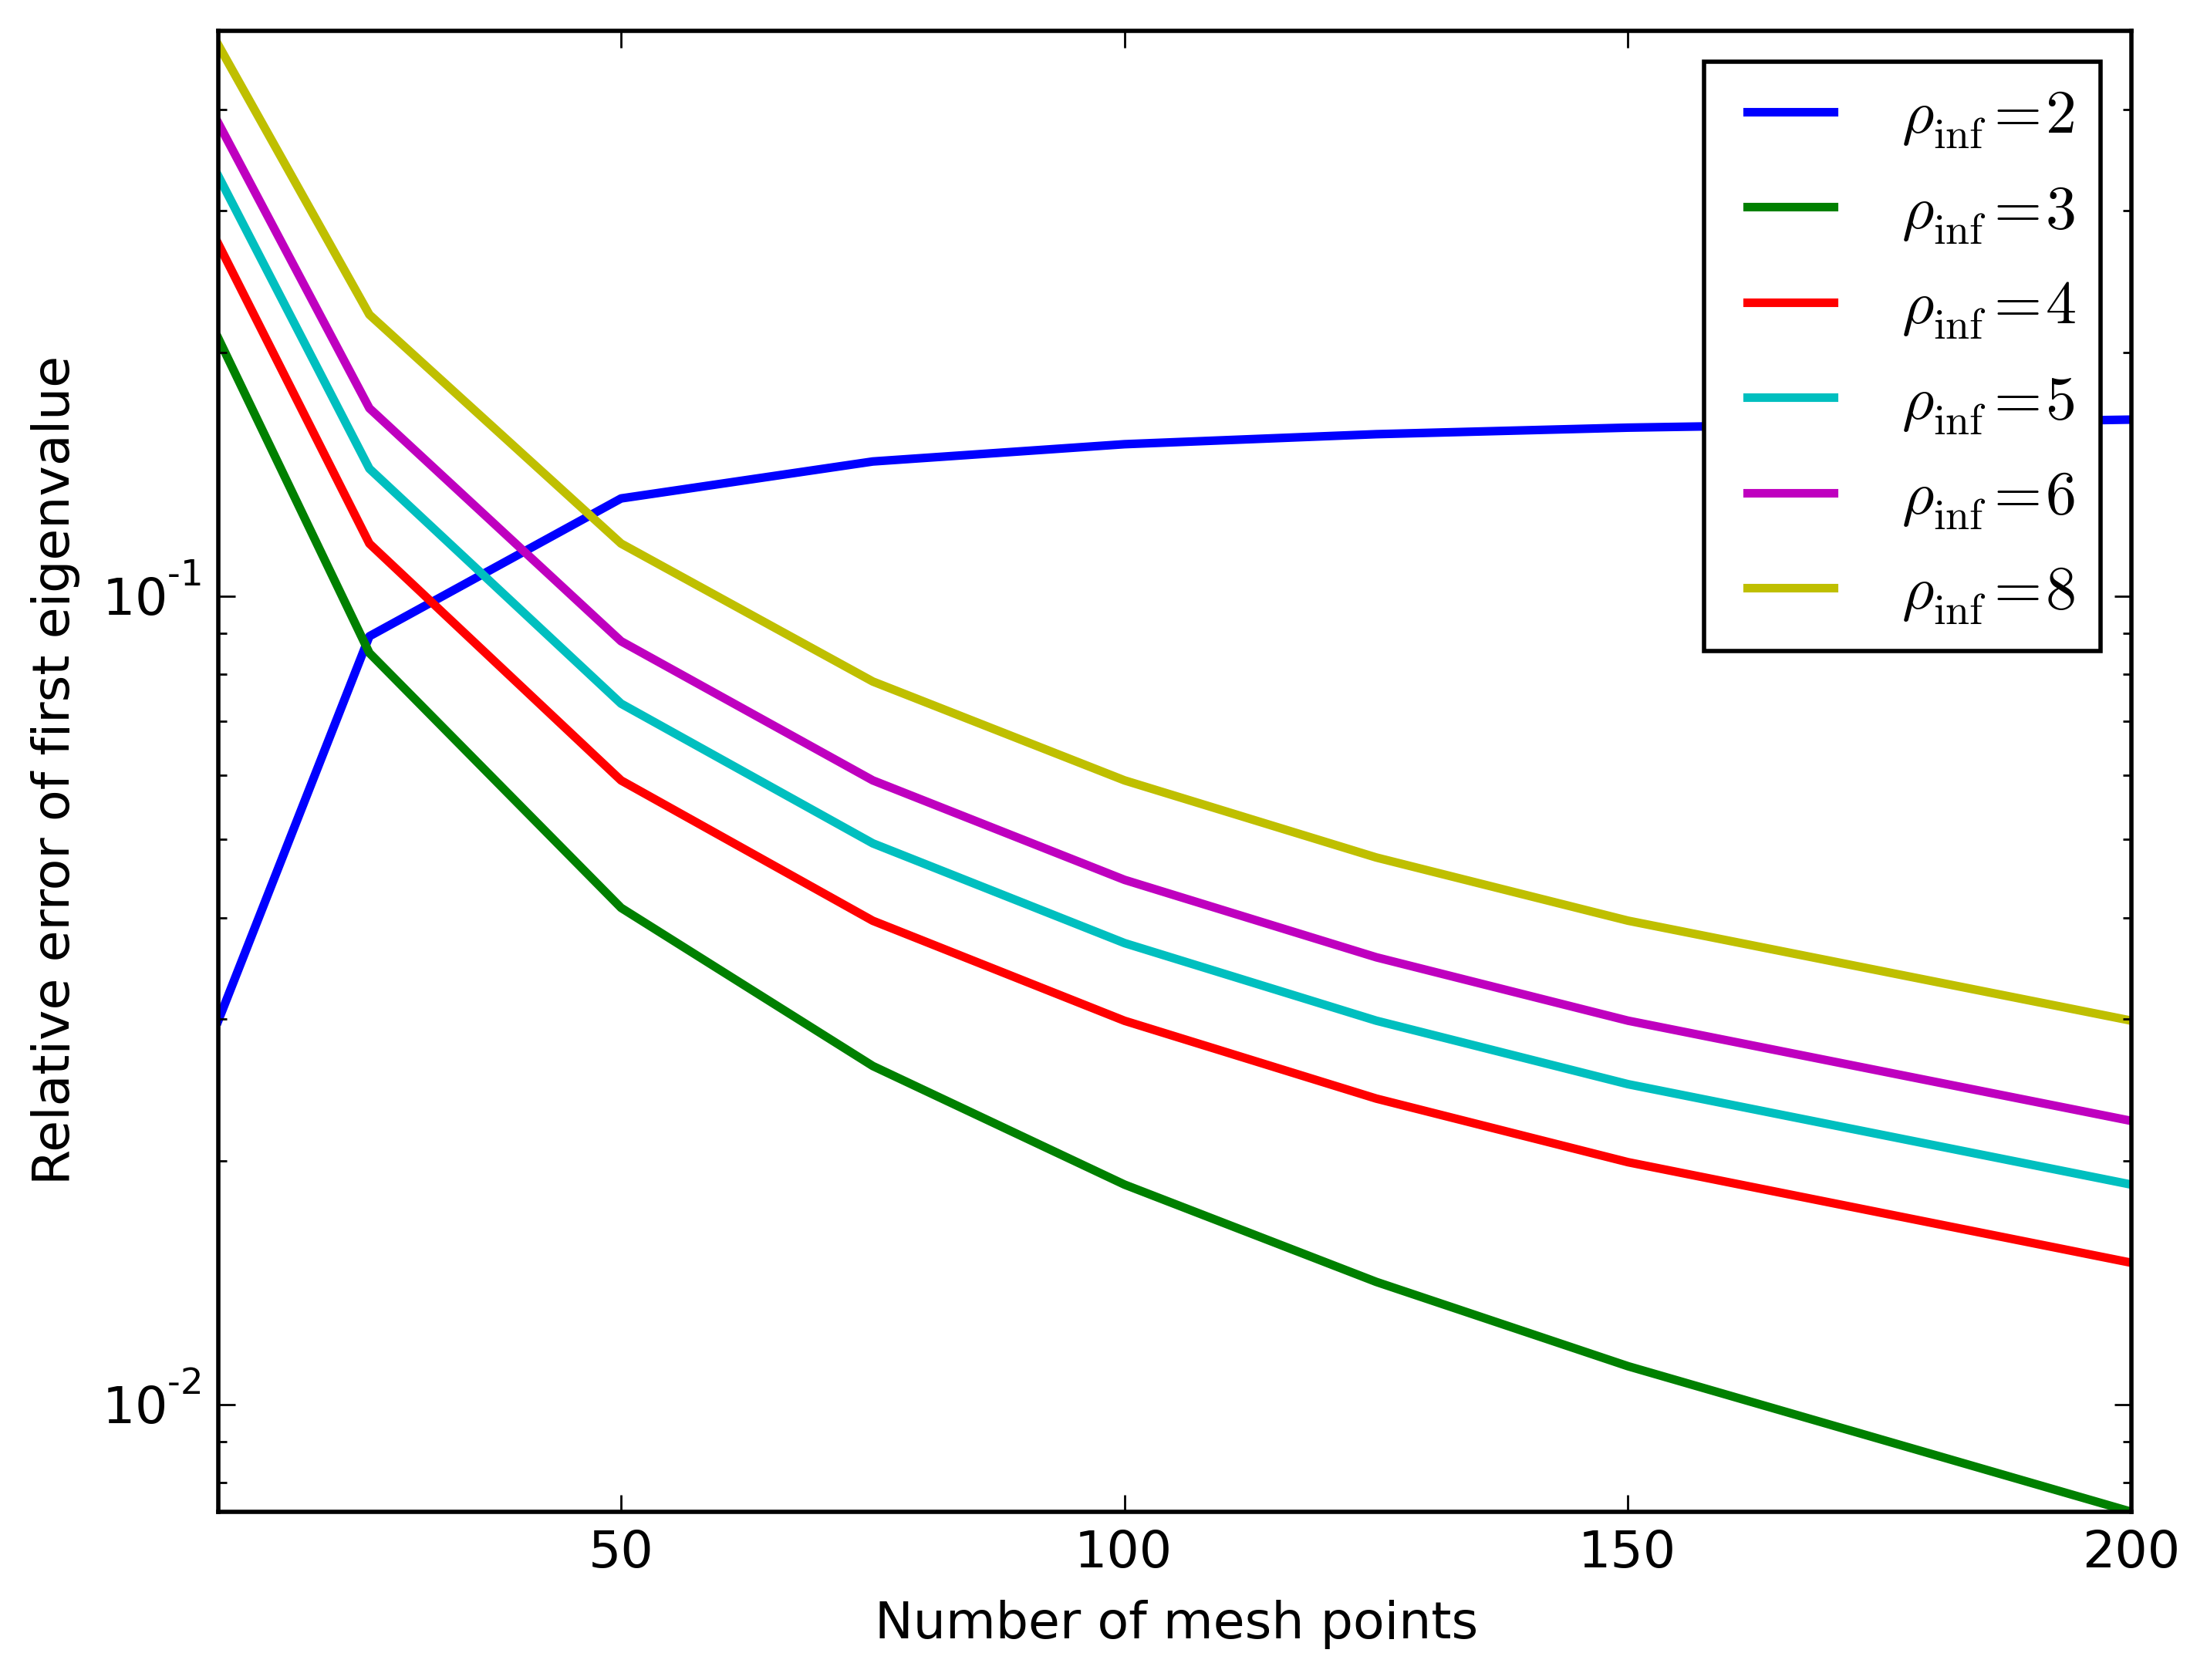
\includegraphics[width=\figurewidth]{../results/rel_logE0.png}
\caption{Relative error in the first energy level for 
different N and $\rho_\infty$}
\label{fig:relE0}
\end{figure}

\begin{figure}
\centering
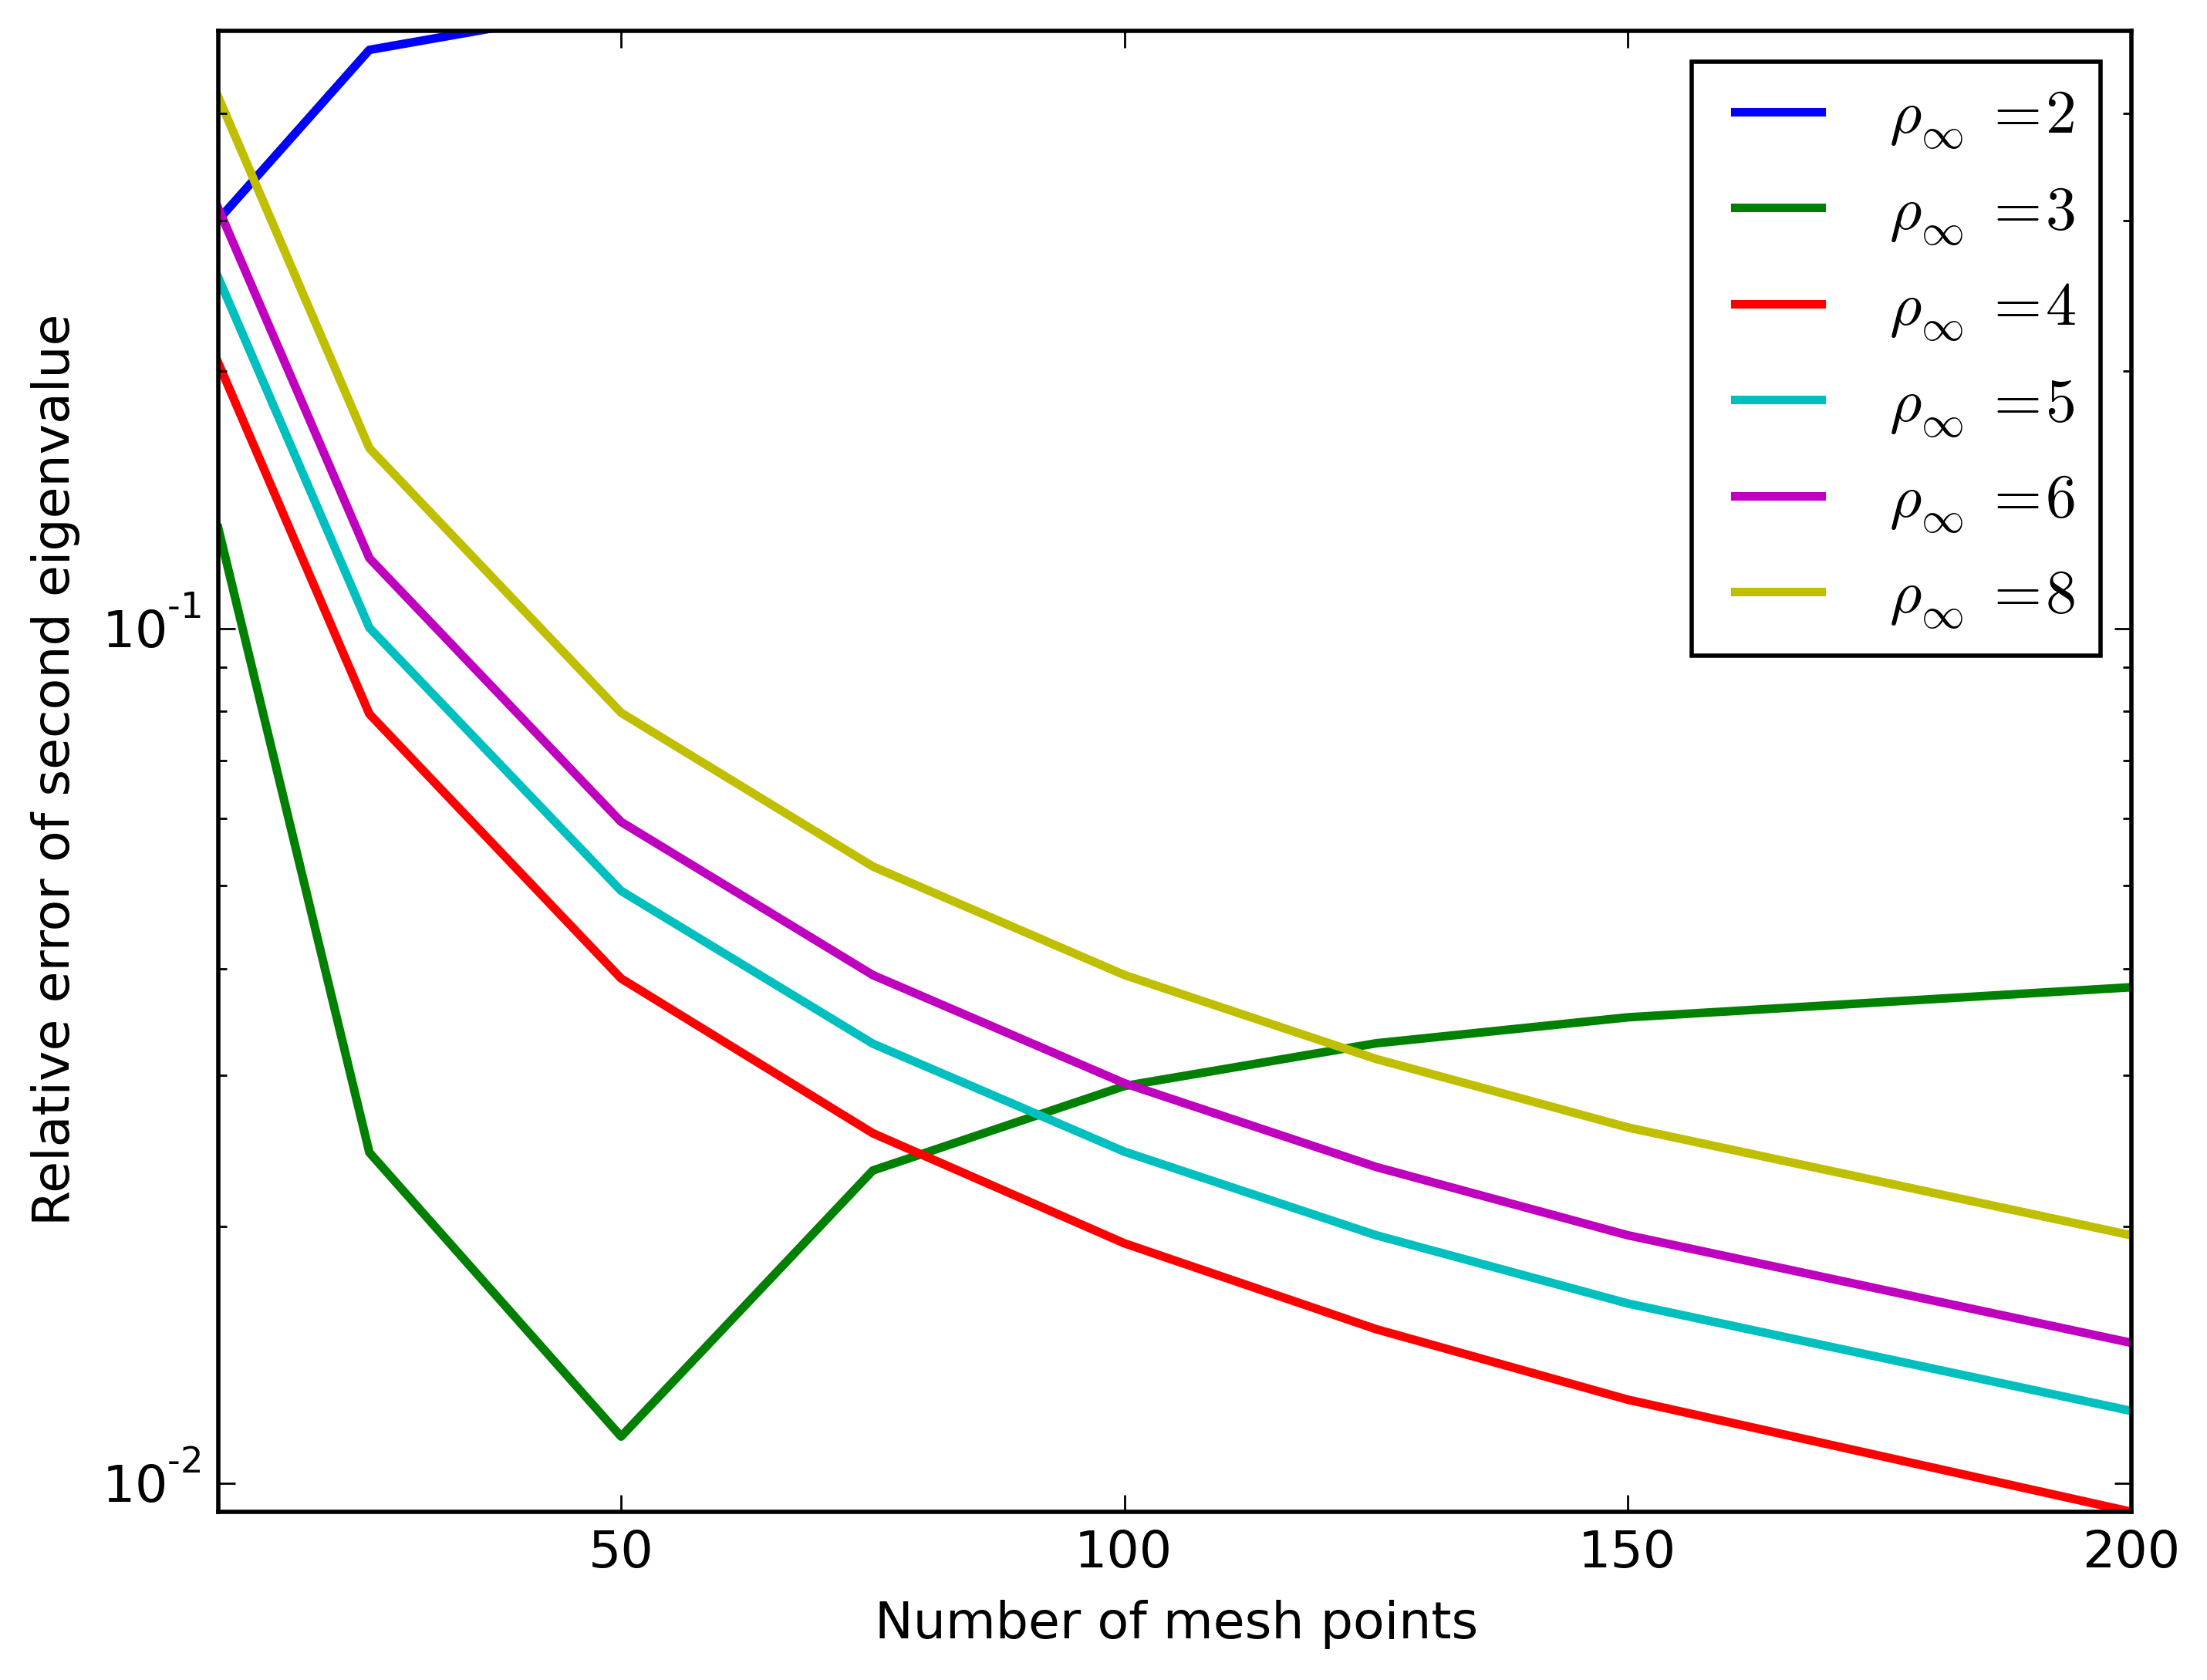
\includegraphics[width=\figurewidth]{../results/rel_logE1.png}
\caption{Relative error in the second energy level for different N,
and $\rho_\infty$}
\label{fig:relE1}
\end{figure}

\begin{figure}
\centering
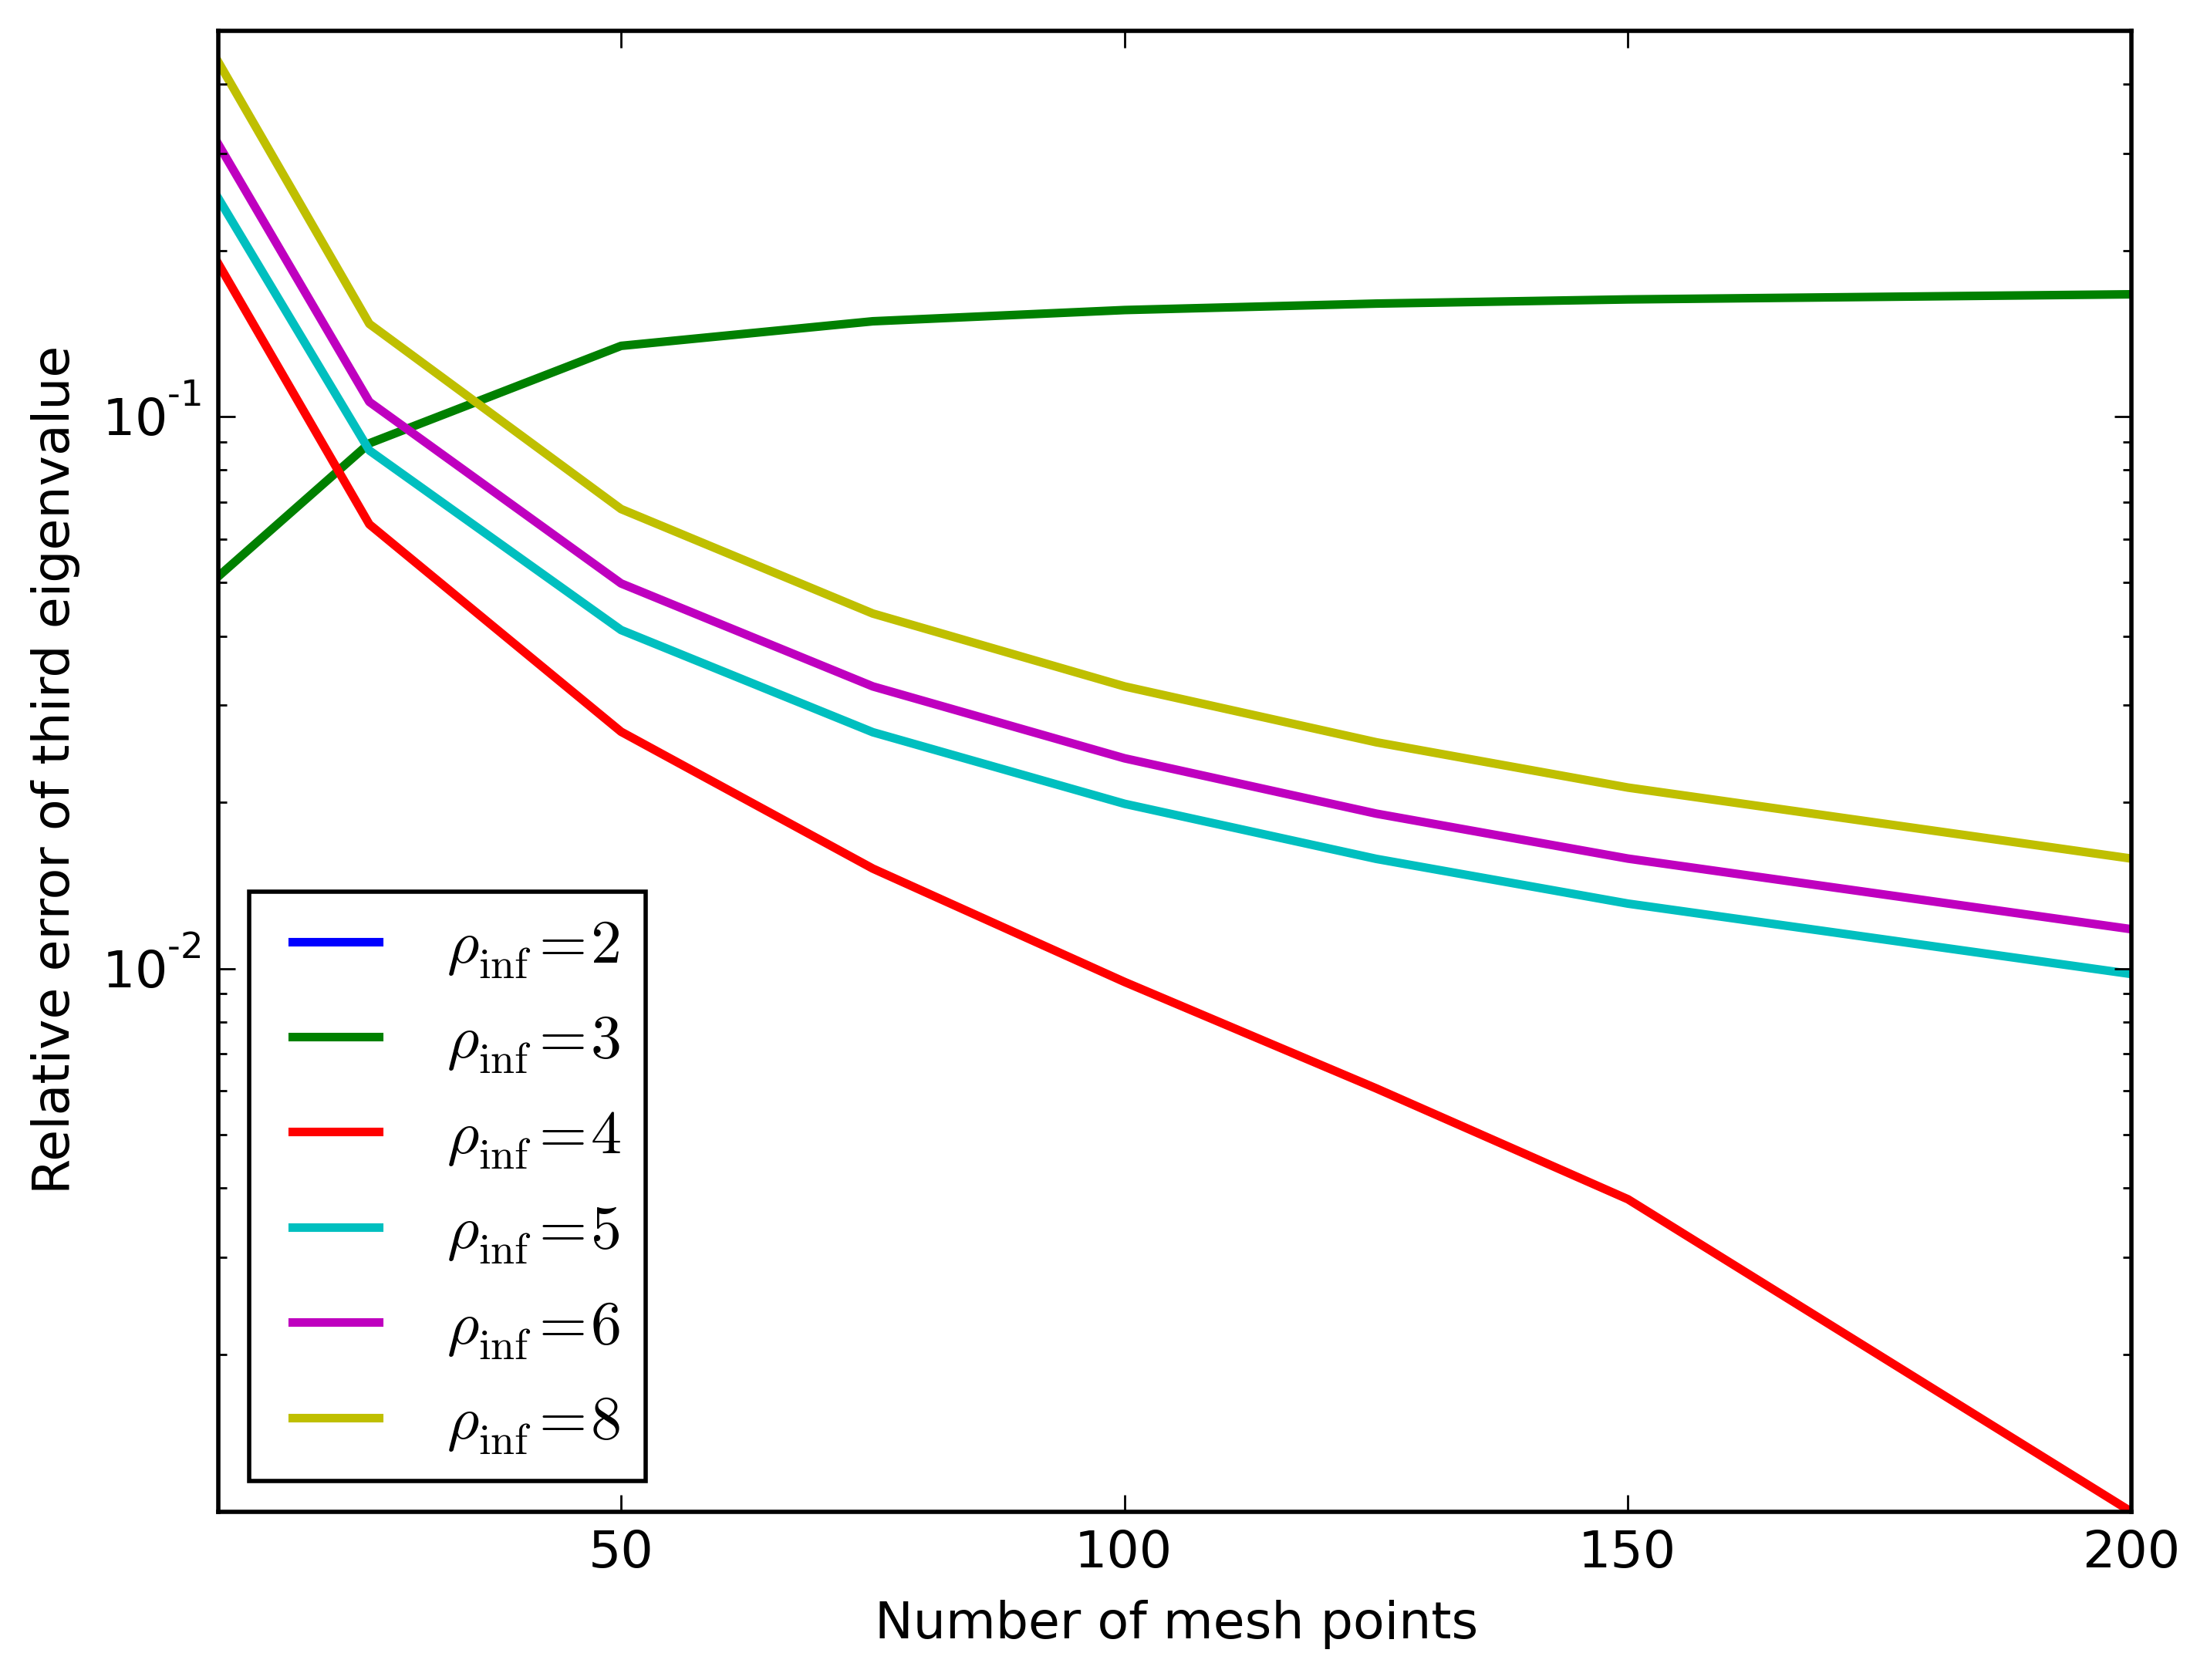
\includegraphics[width=\figurewidth]{../results/rel_logE2.png}
\caption{Relative error in the third energy level for different N,
and $\rho_\infty$}
\label{fig:relE2}
\end{figure}

\subsubsection{Wave function}

The wave function is found by squaring the eigenvectors found for the 
Hamiltonian. The three lowest wave functions have been selected and
plotted for different values of $\rho_\infty$,
\ref{fig:psi0rho}, \ref{fig:psi1rho}, \ref{fig:psi2rho} and 
different values of N, \ref{fig:psi0N}, \ref{fig:psi1N} and 
\ref{fig:psi2N}.

When N is increased the solutions tends to decrease and get smoother.
This decrease is due to a better approximation of the integral for 
larger N.

The different values of $\rho_\infty$ gives different eigenvectors.
If it is chosen to low, the wave function will have a cutoff, and some 
of the true behaviour may be lost.


\begin{figure}
\centering
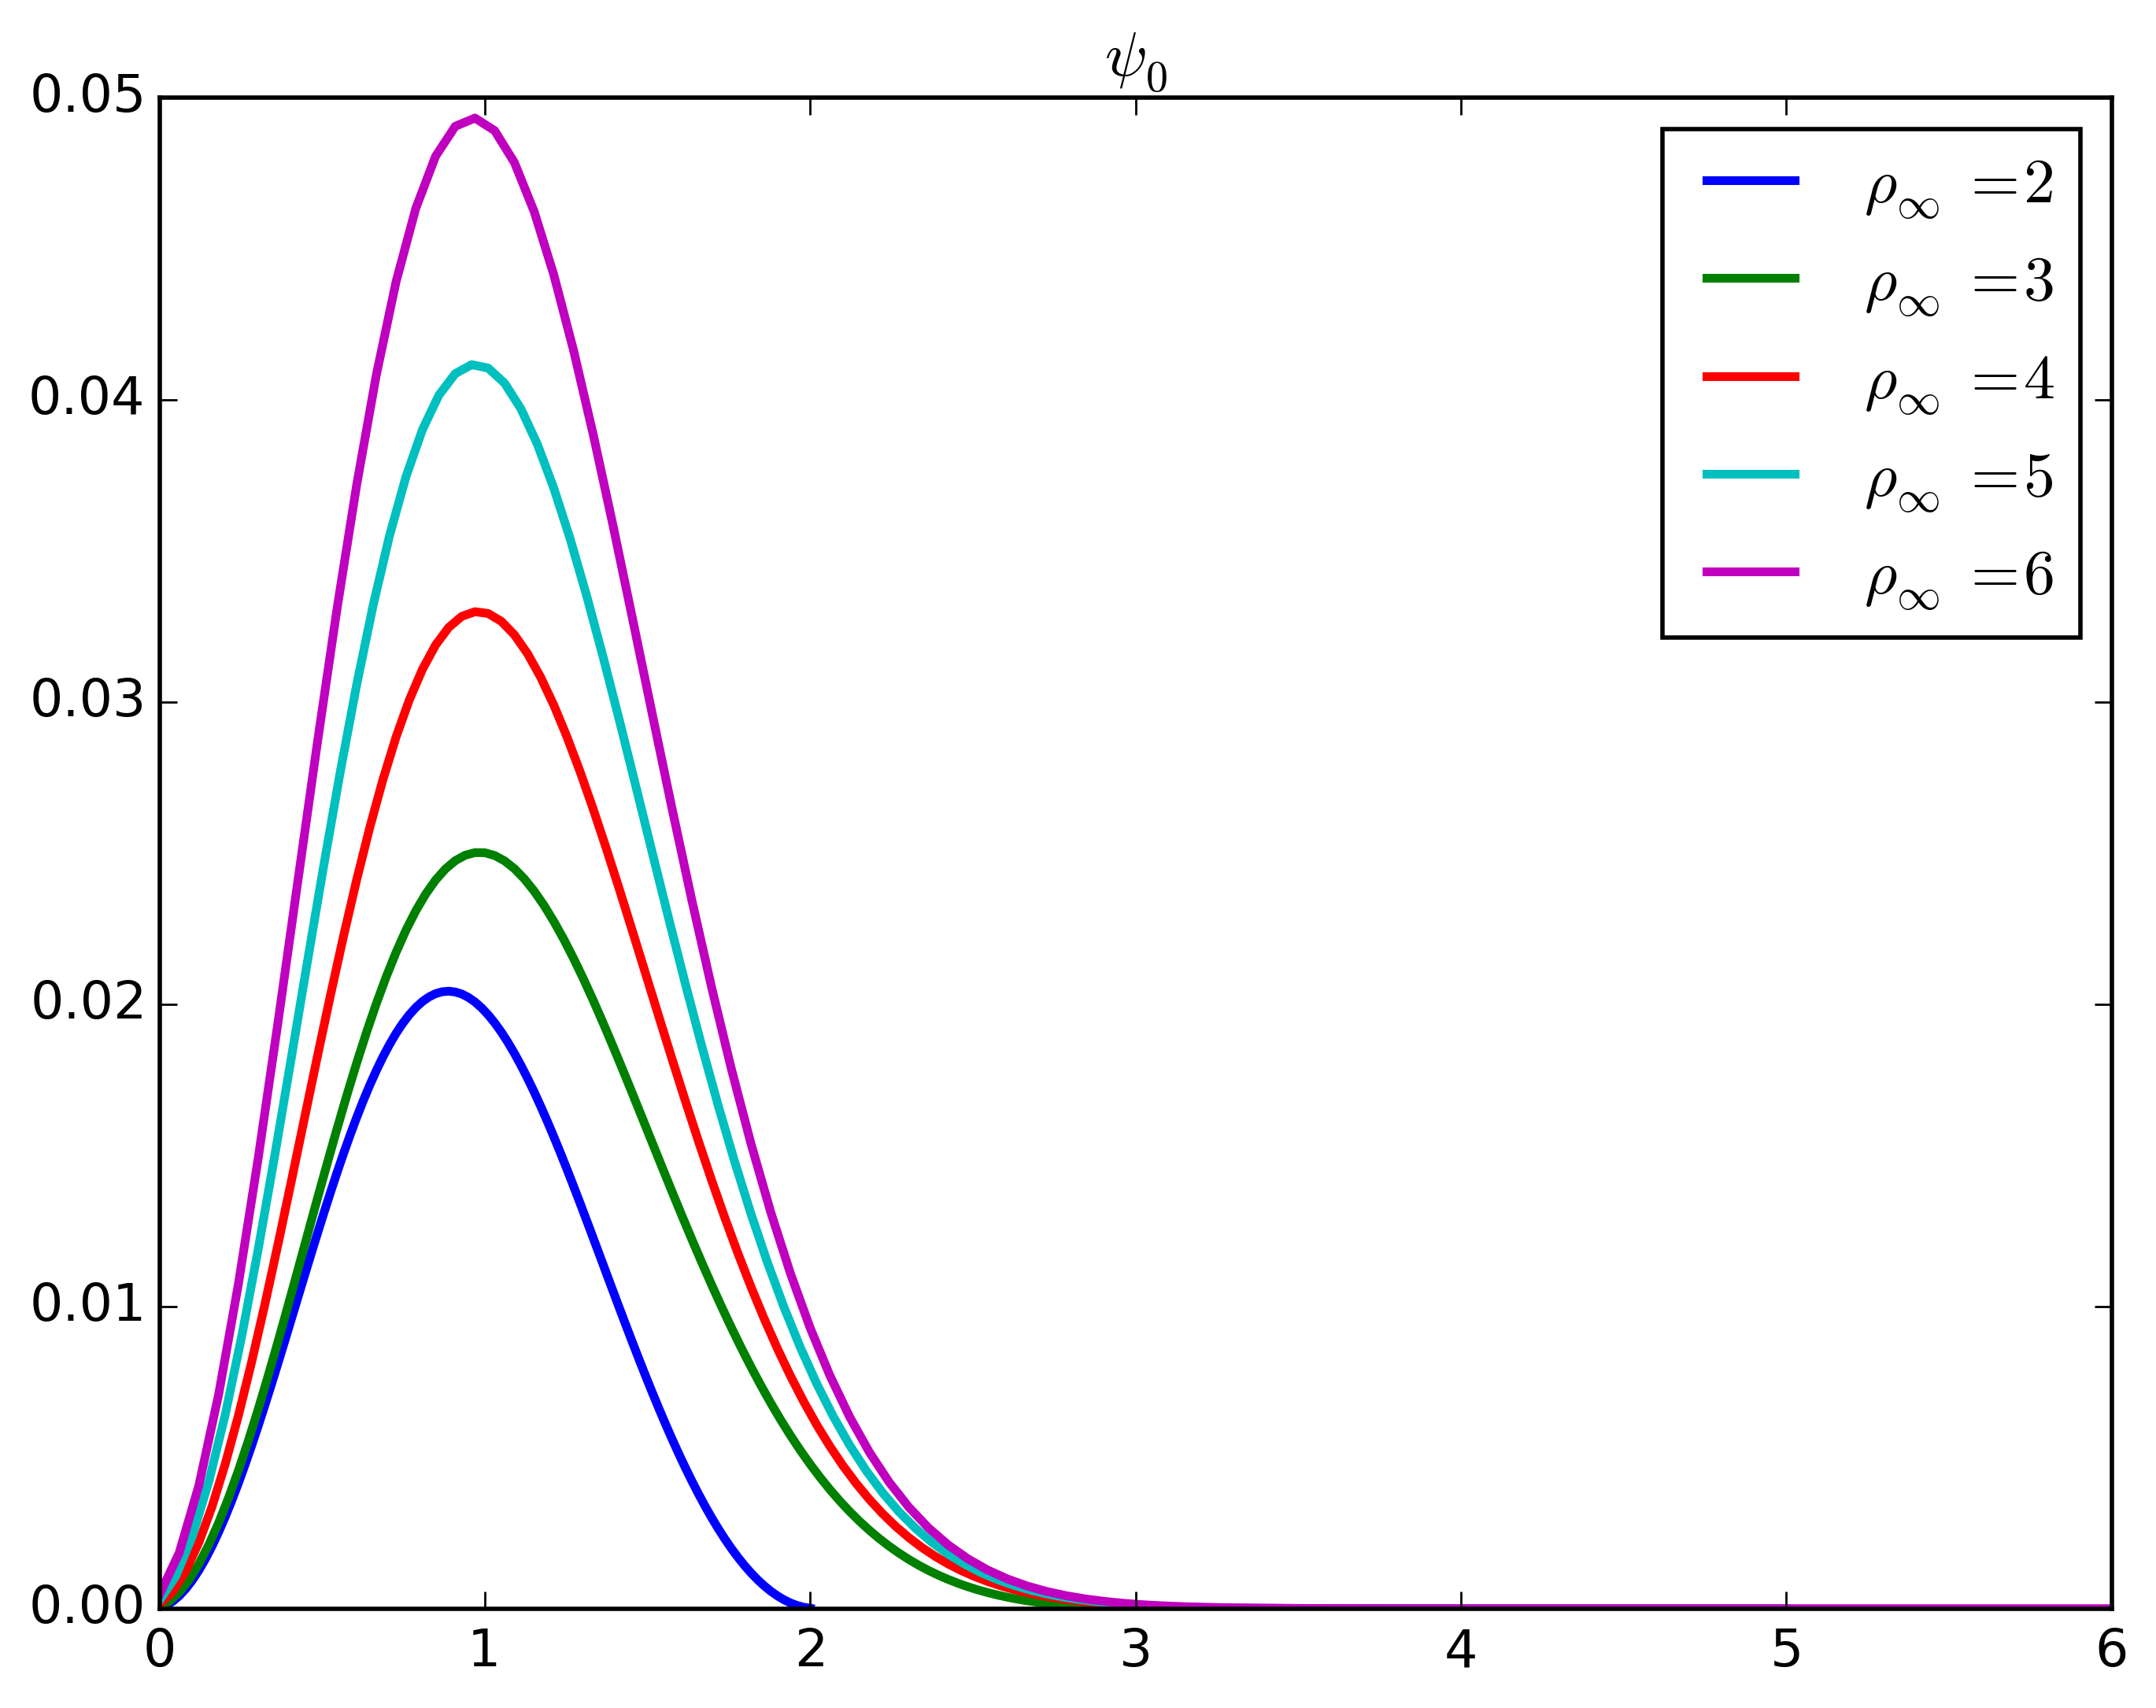
\includegraphics[width=\figurewidth]{../results/psi_inf_compare_psi0.png}
\caption{Wave function for different values of $\rho_\infty$ for
the eigenvector associated with the lowest energy}
\label{fig:psi0rho}
\end{figure}

\begin{figure}
\centering
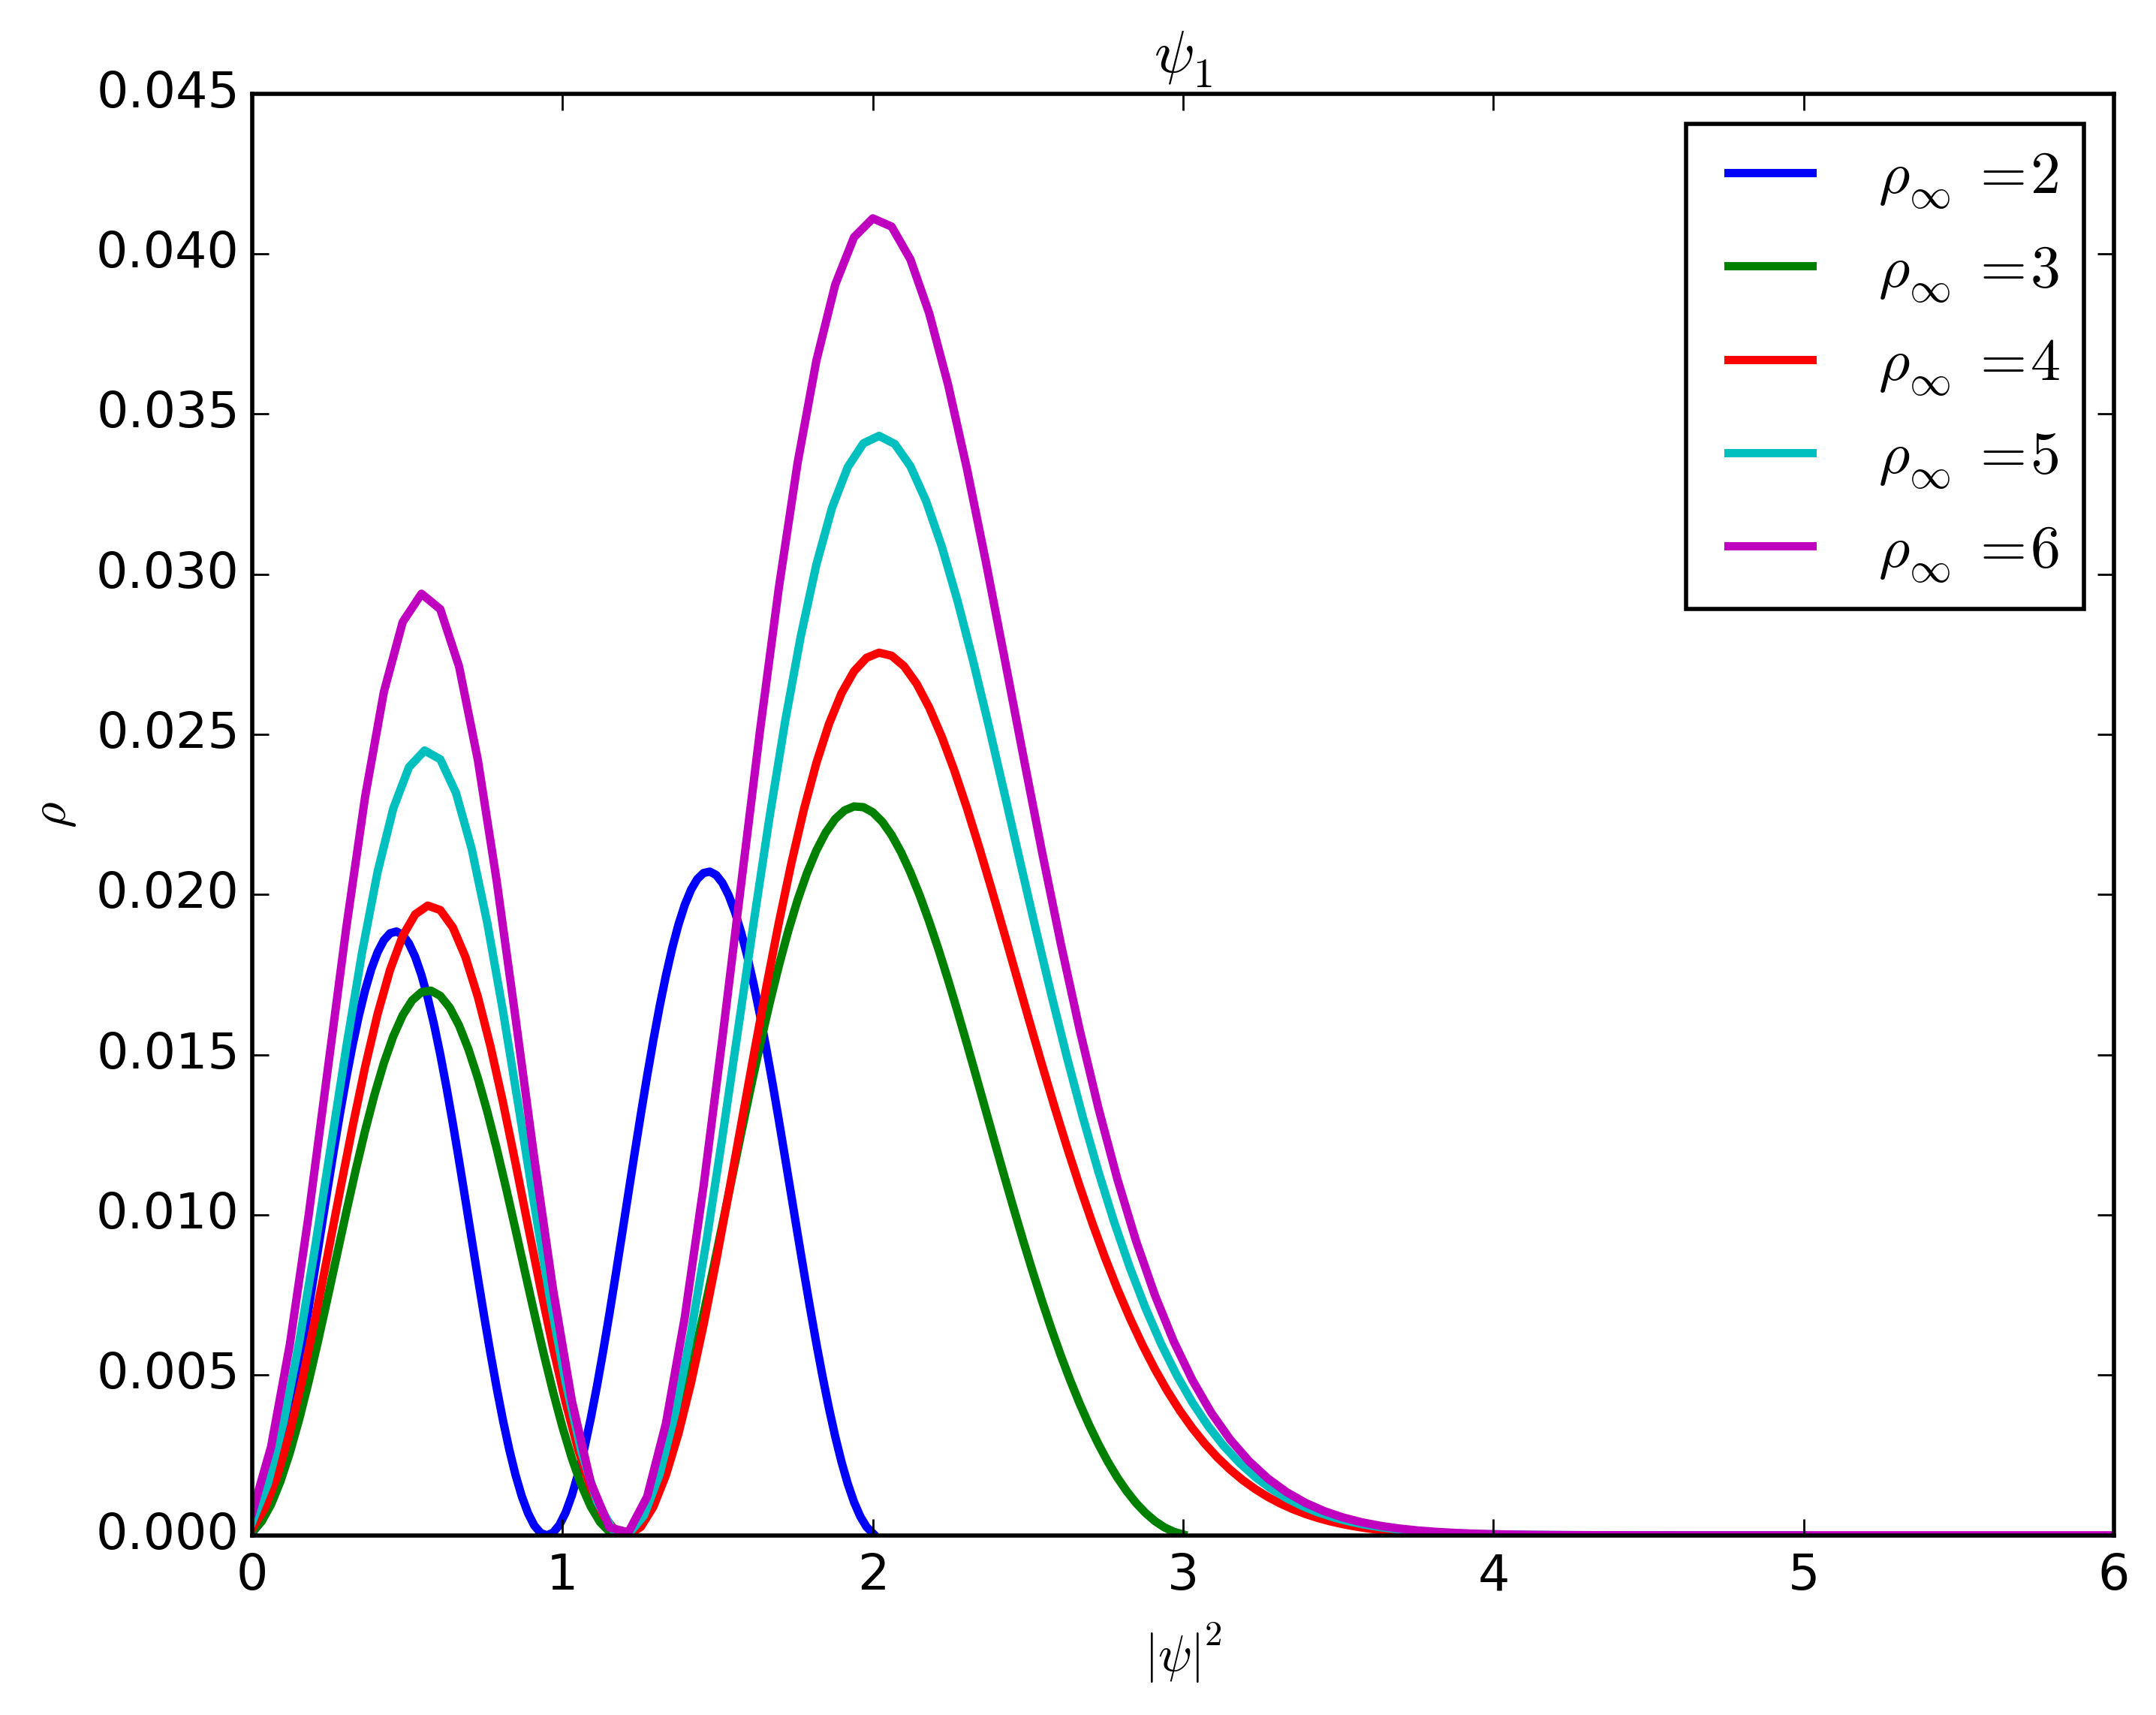
\includegraphics[width=\figurewidth]{../results/psi_inf_compare_psi1.png}
\caption{Wave function for different values of $\rho_\infty$ for
the eigenvector associated with the second lowest energy}
\label{fig:psi1rho}
\end{figure}

\begin{figure}
\centering
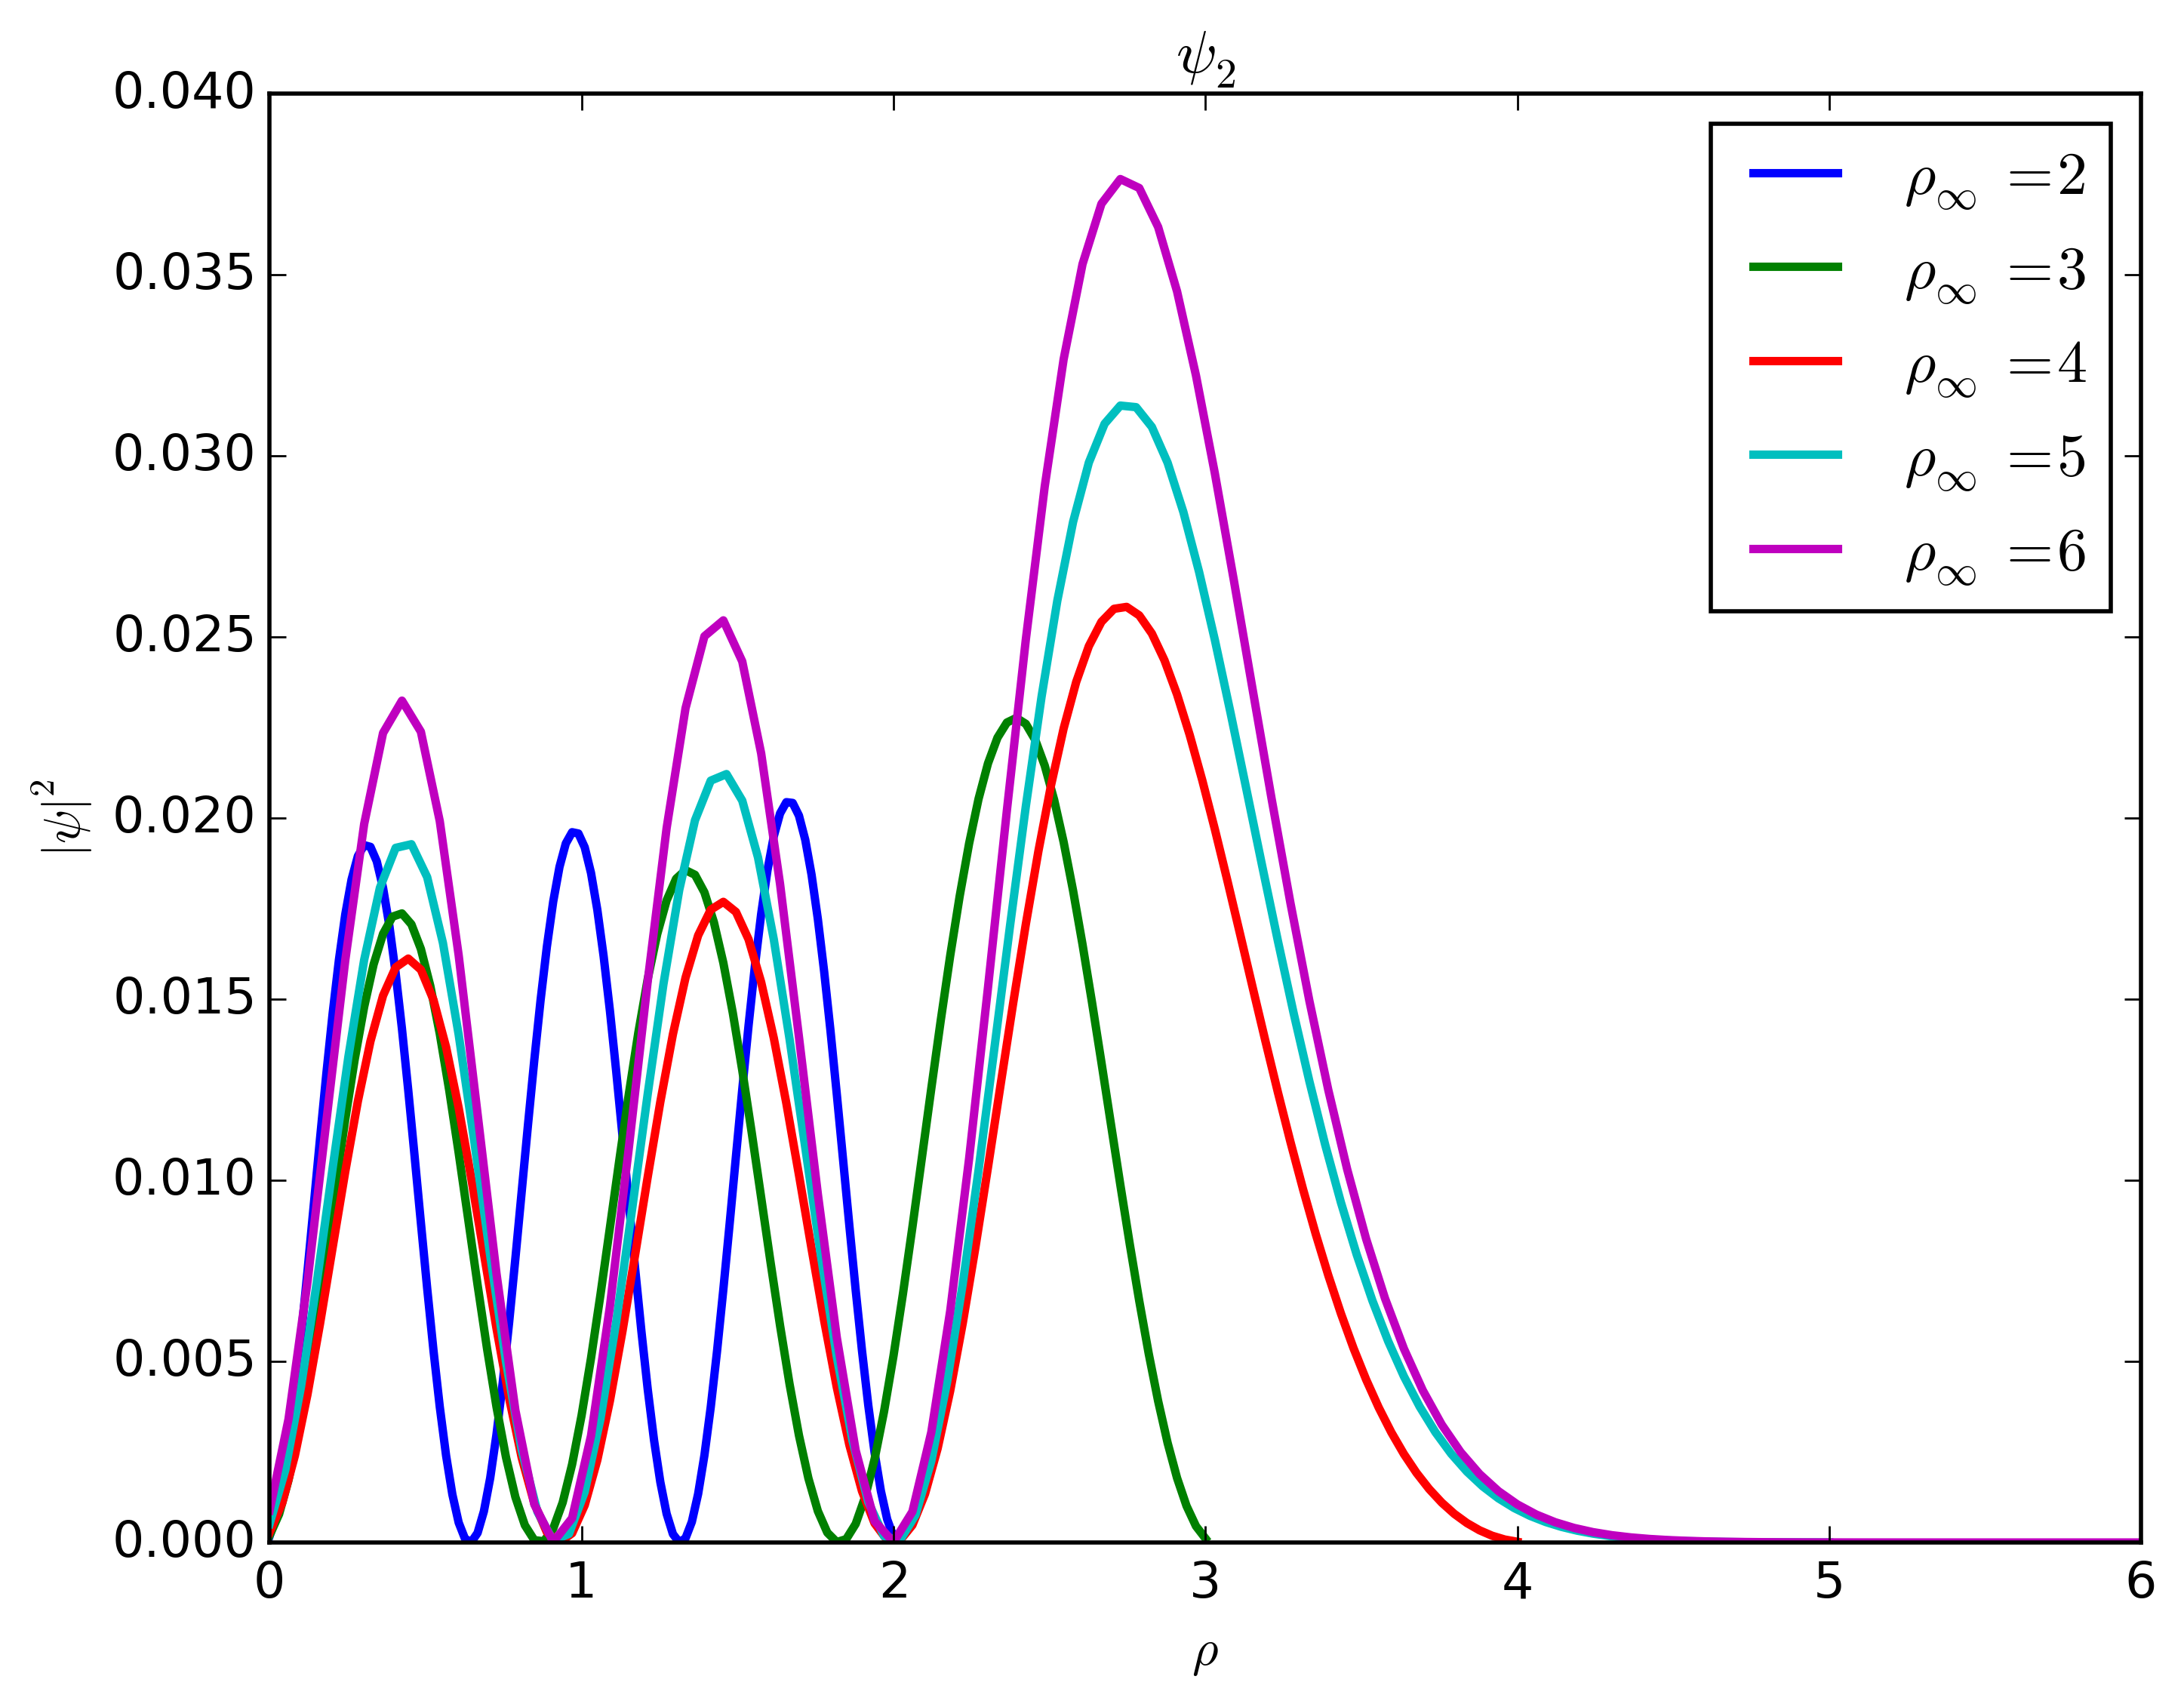
\includegraphics[width=\figurewidth]{../results/psi_inf_compare_psi2.png}
\caption{Wave function for different values of $\rho_\infty$ for
the eigenvector associated with the third lowest energy}
\label{fig:psi2rho}
\end{figure}

\begin{figure}
\centering
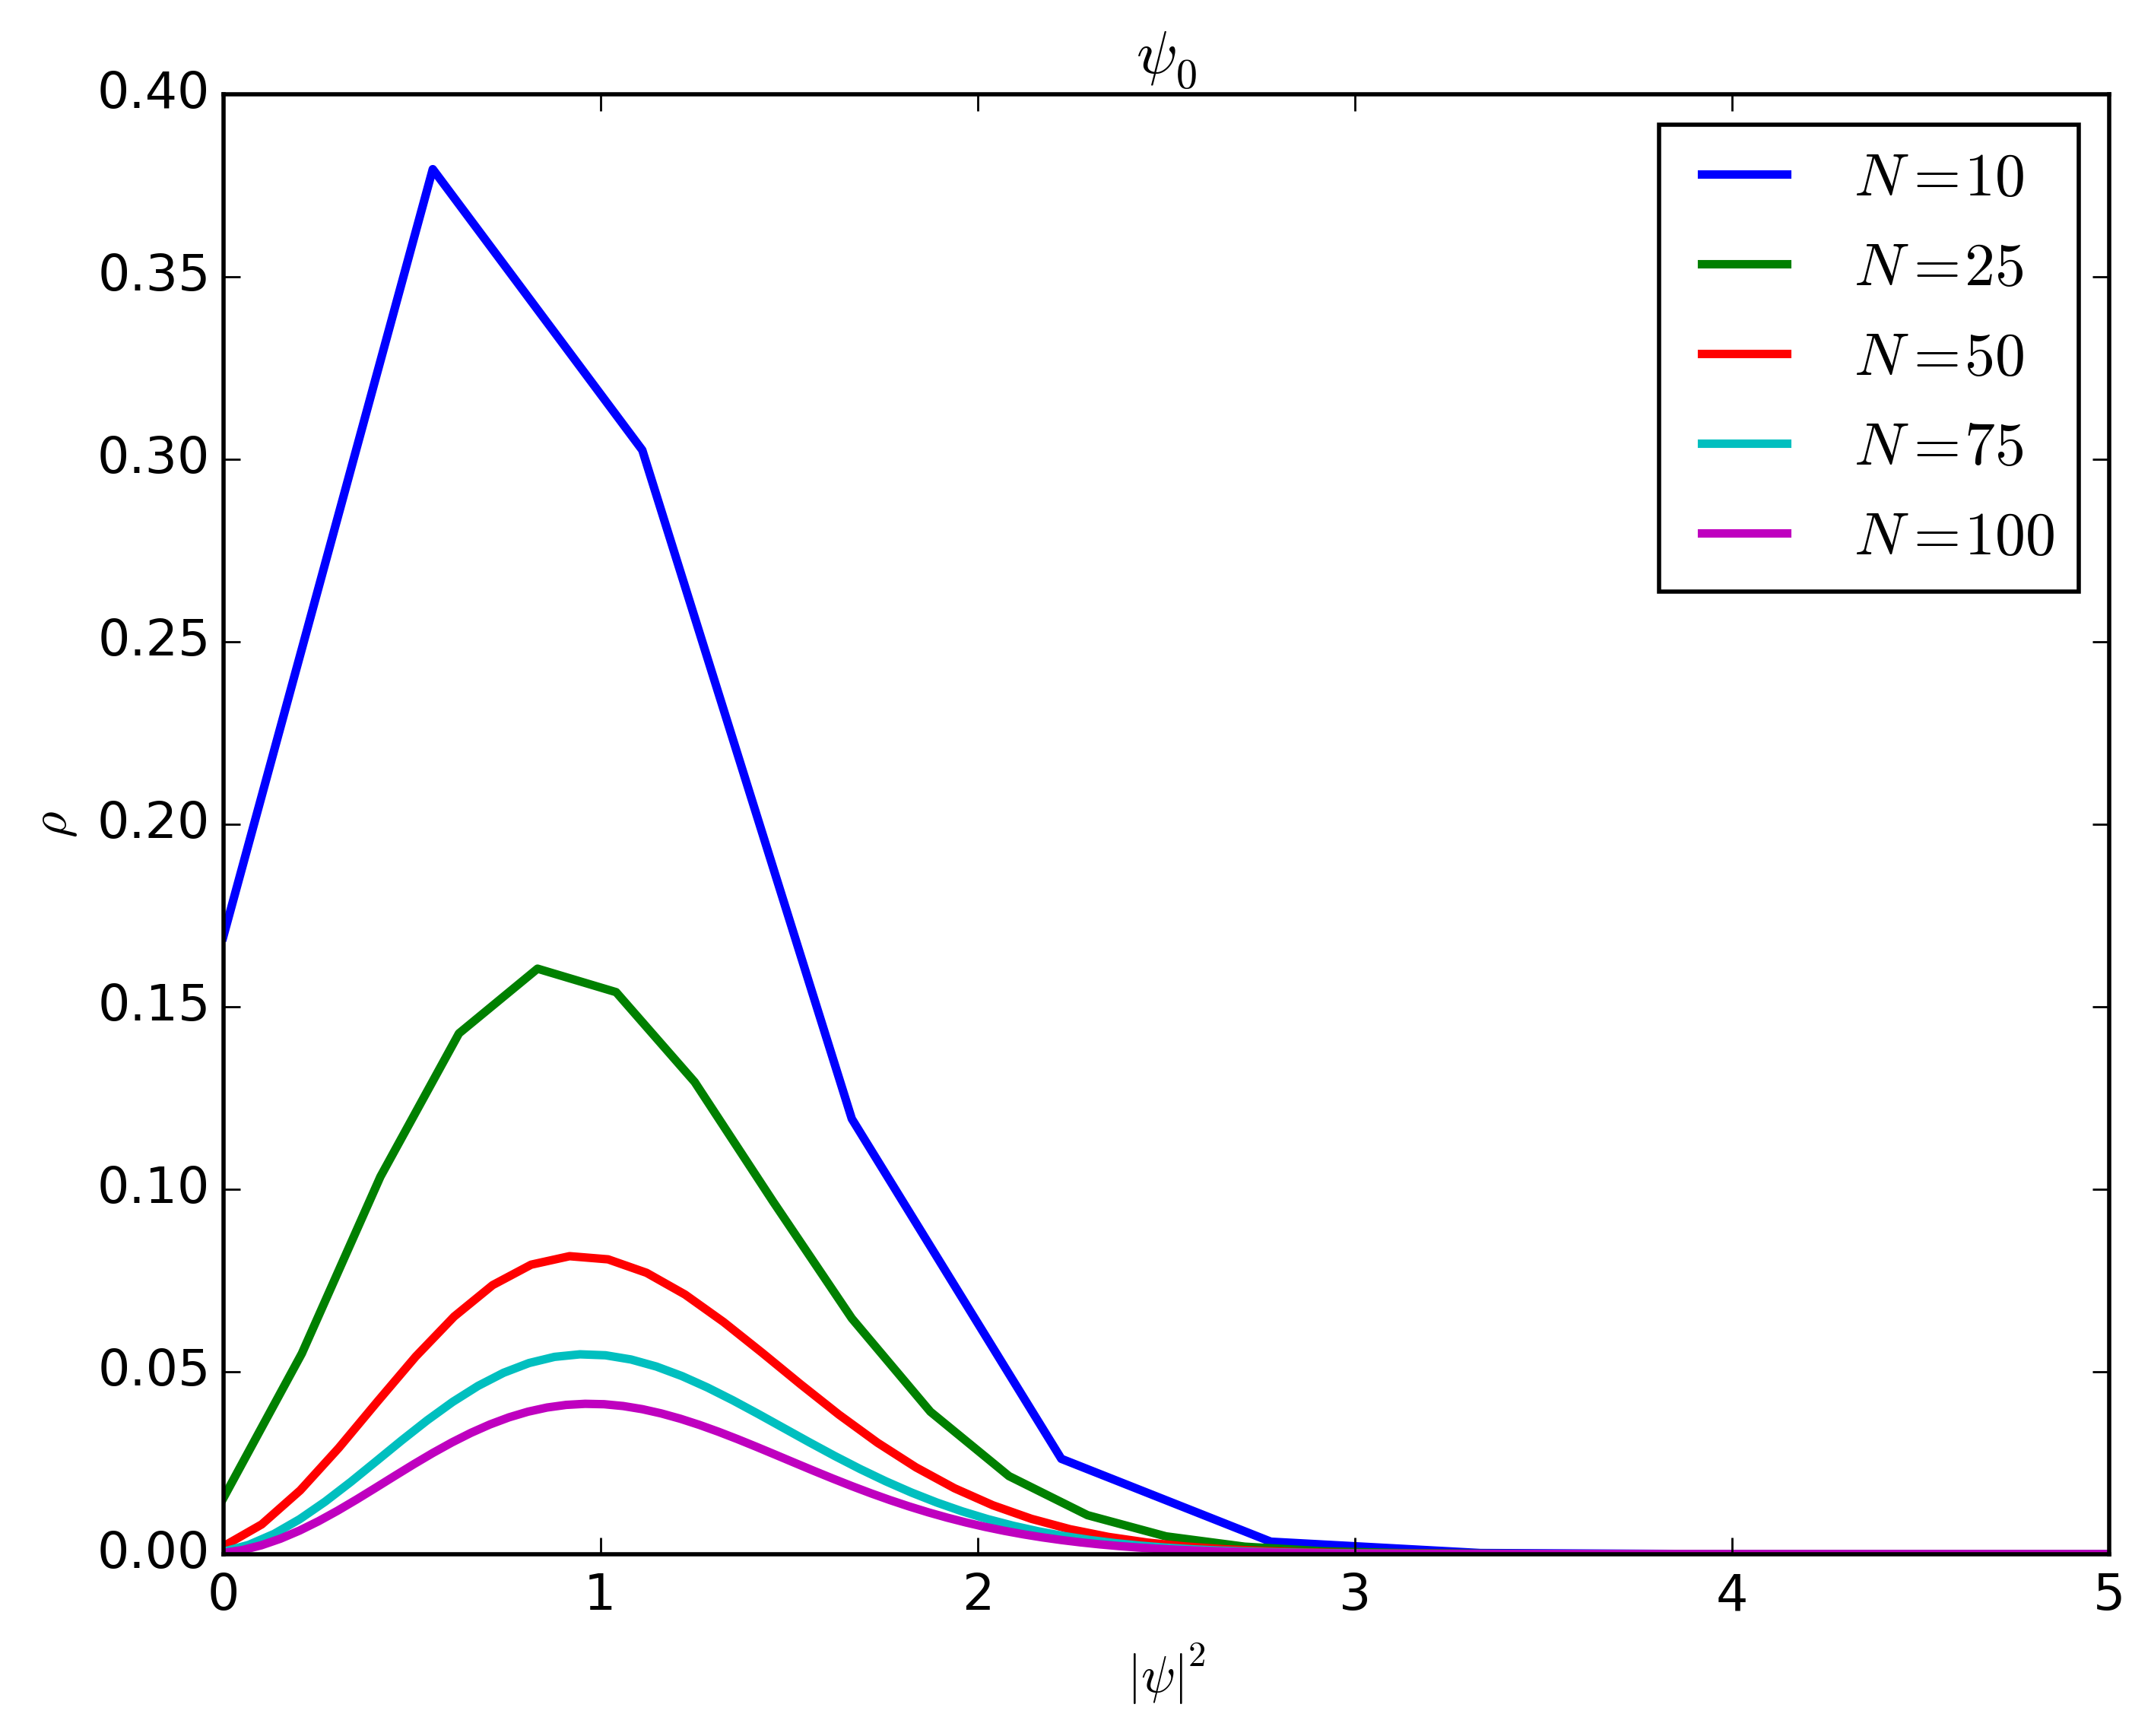
\includegraphics[width=\figurewidth]{../results/N_compare_psi0.png}
\caption{Wave function for different values of $N$ for
the eigenvector associated with the lowest energy}
\label{fig:psi0N}
\end{figure}

\begin{figure}
\centering
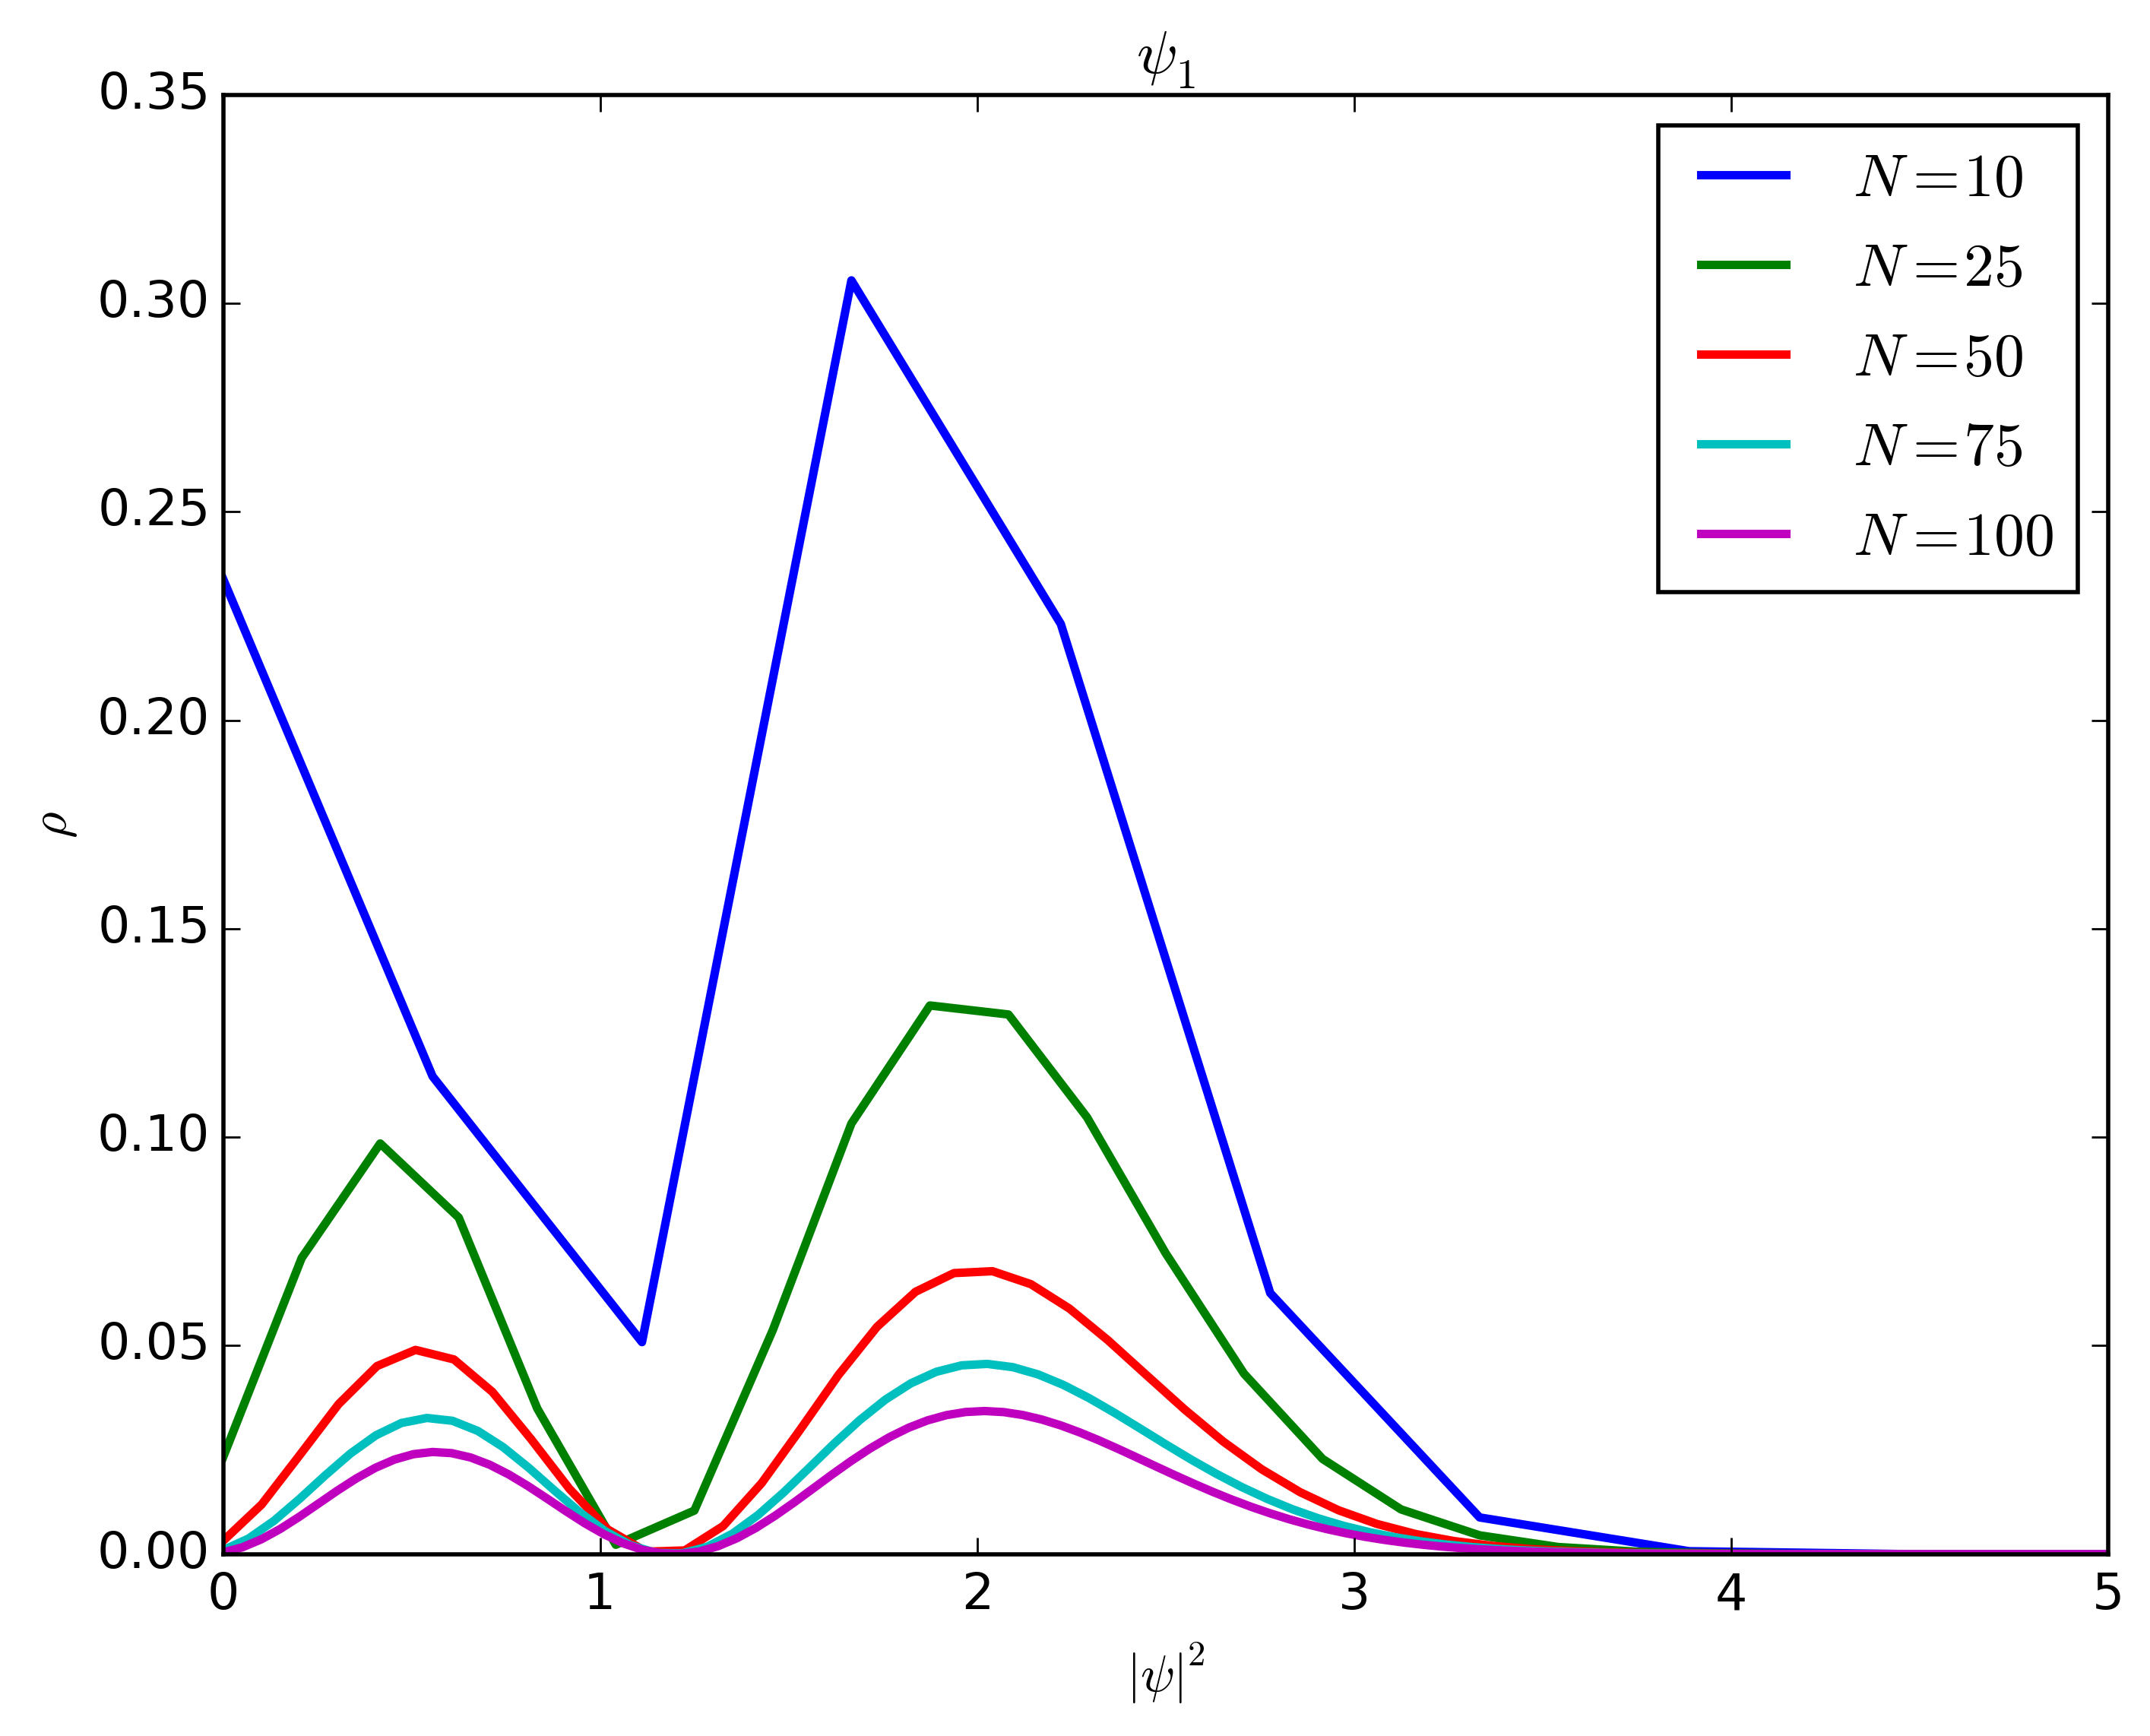
\includegraphics[width=\figurewidth]{../results/N_compare_psi1.png}
\caption{Wave function for different values of $N$ for
the eigenvector associated with the second lowest energy}
\label{fig:psi1N}
\end{figure}

\begin{figure}
\centering
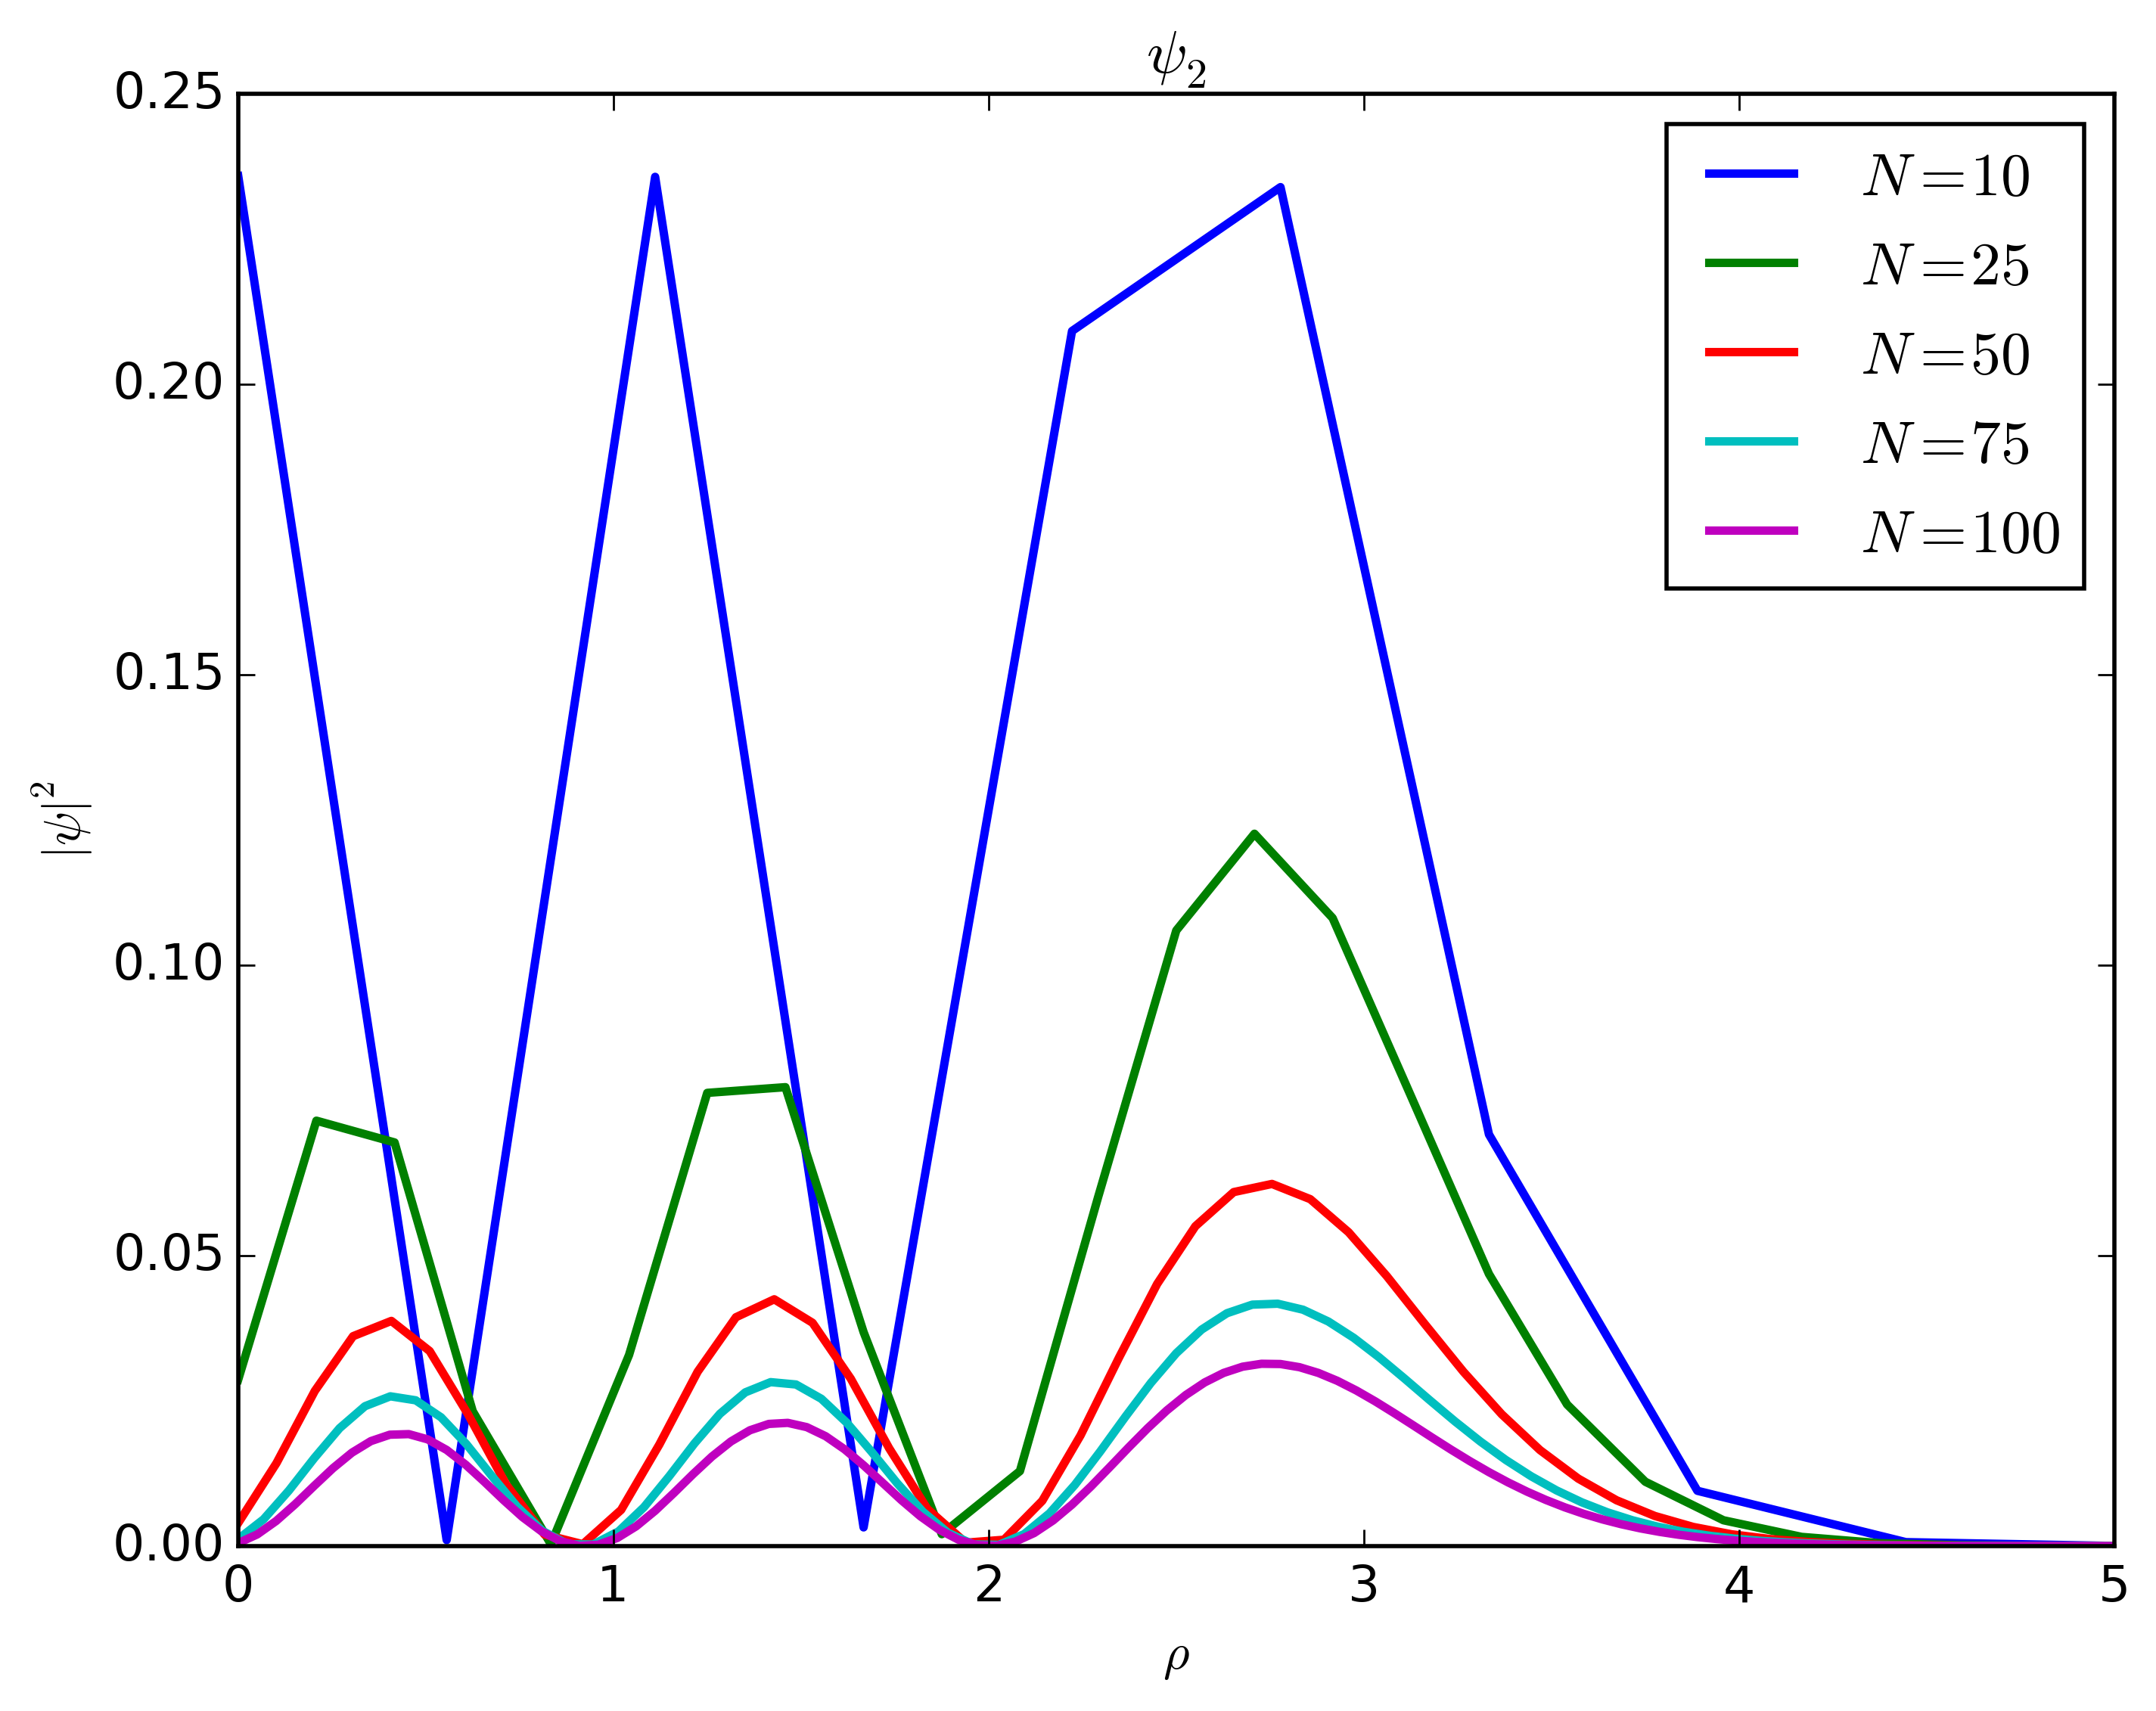
\includegraphics[width=\figurewidth]{../results/N_compare_psi2.png}
\caption{Wave function for different values of $N$ for
the eigenvector associated with the third lowest energy}
\label{fig:psi2N}
\end{figure}

\subsection{Two electrons}

For a selection of $\omega_r$ with $N = 100$ and $\rho_\infty = 6$ we
obtain the plots \ref{fig:omegar0}, \ref{fig:omegar1} and 
\ref{fig:omegar2} for the three lowest eigenvalues. The 

\subsection{Reproduction of results}





\begin{figure}
\centering
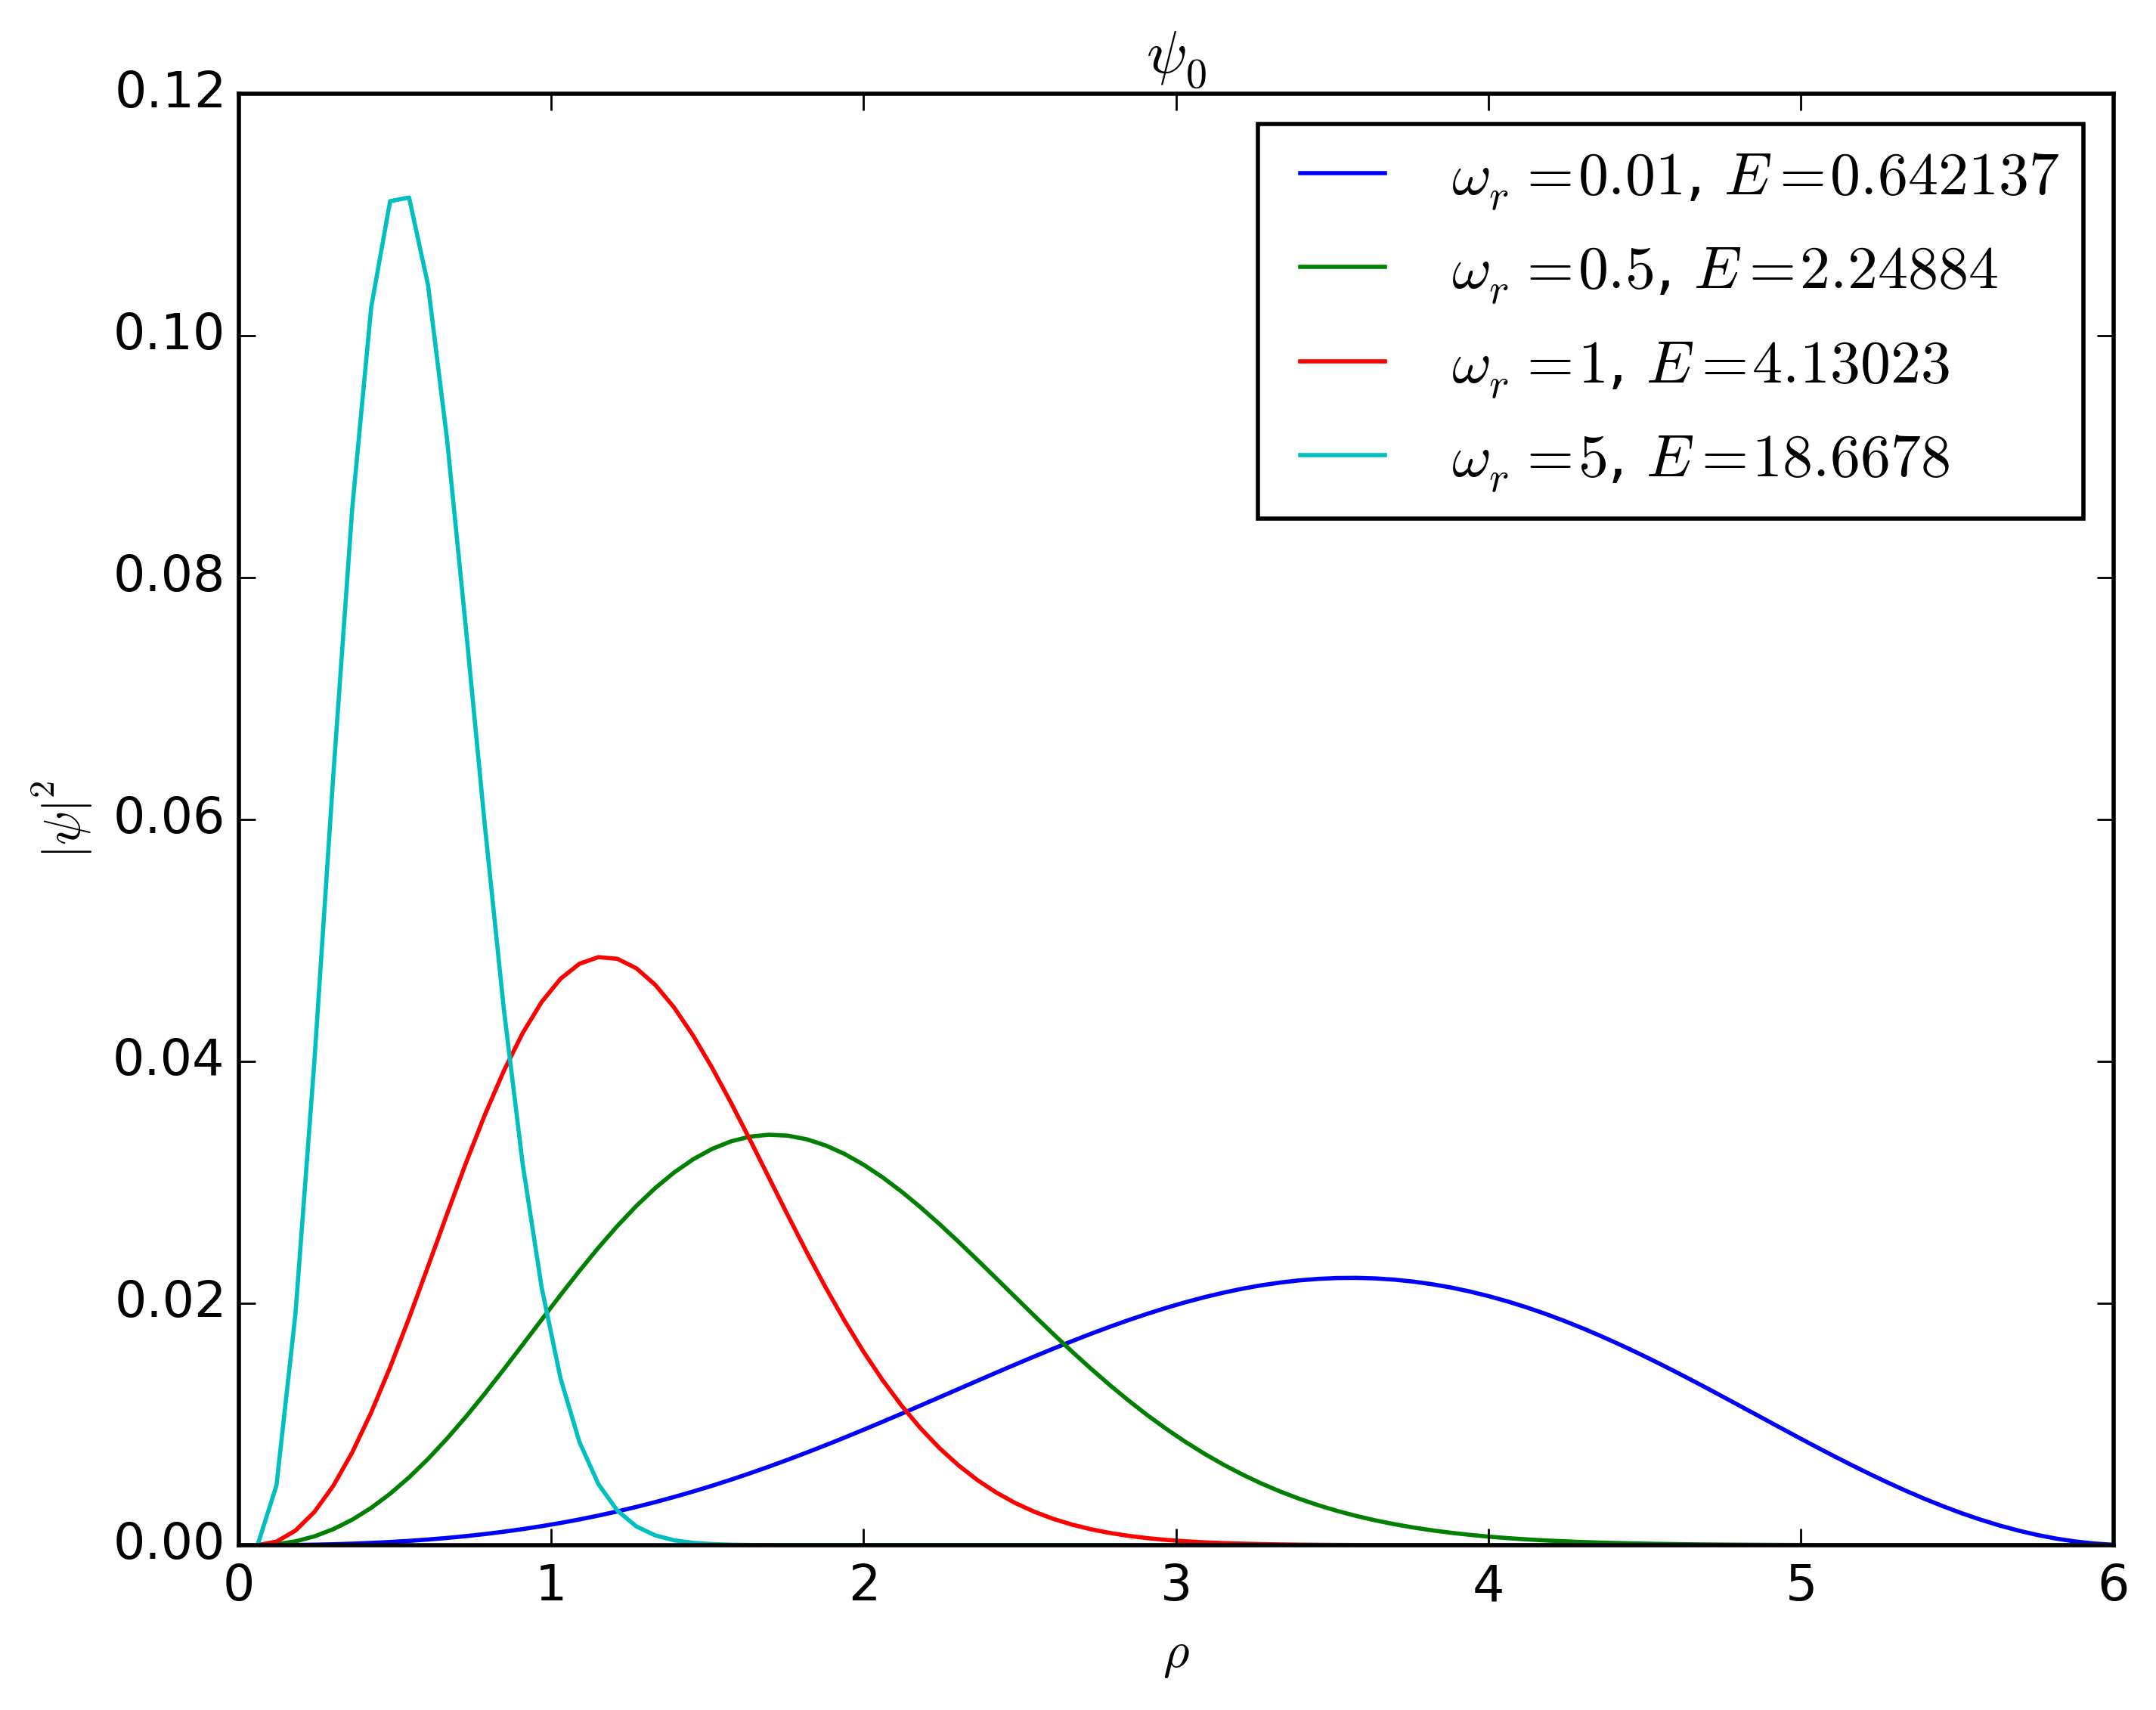
\includegraphics[width=\figurewidth]{../results/psi_compare_omegar0.png}
\caption{Wave function with lowest energy eigenvalue
for different values of $\omega_r$}
\label{fig:omegar0}
\end{figure}

\begin{figure}
\centering
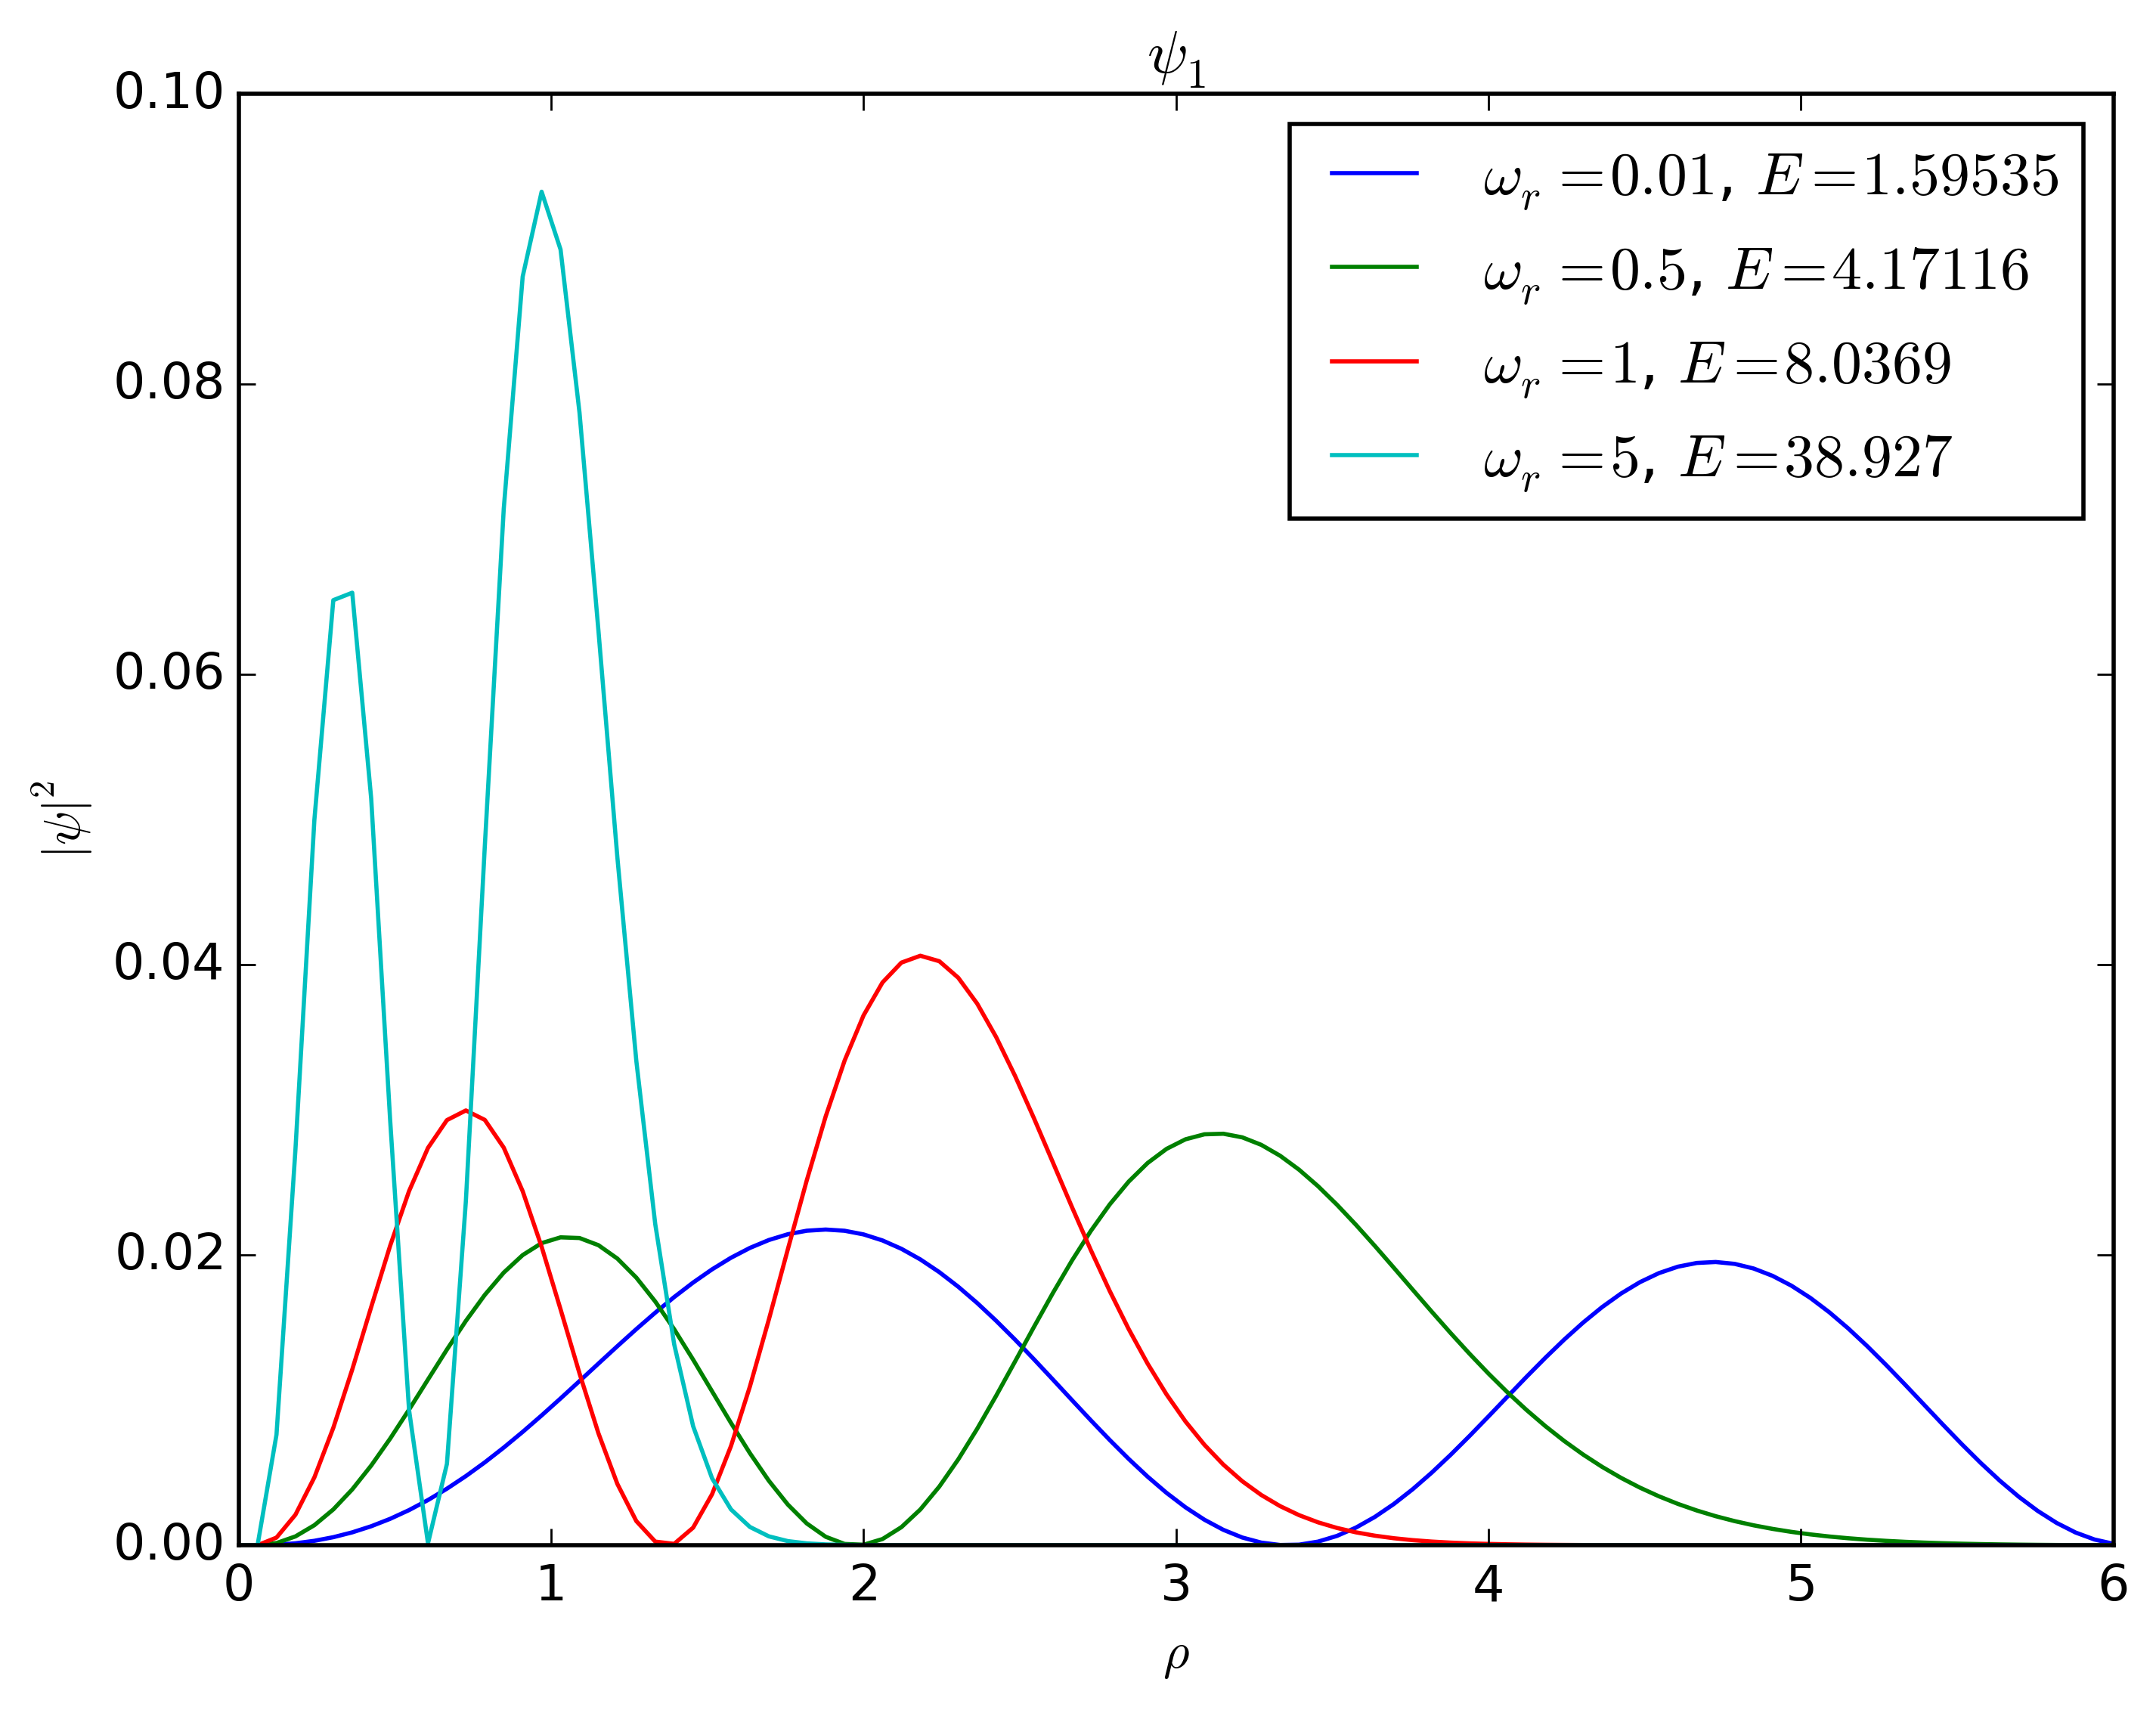
\includegraphics[width=\figurewidth]{../results/psi_compare_omegar1.png}
\caption{Wave function with second lowest energy eigenvalue
for different values of $\omega_r$}
\label{fig:omegar1}
\end{figure}


\begin{figure}
\centering
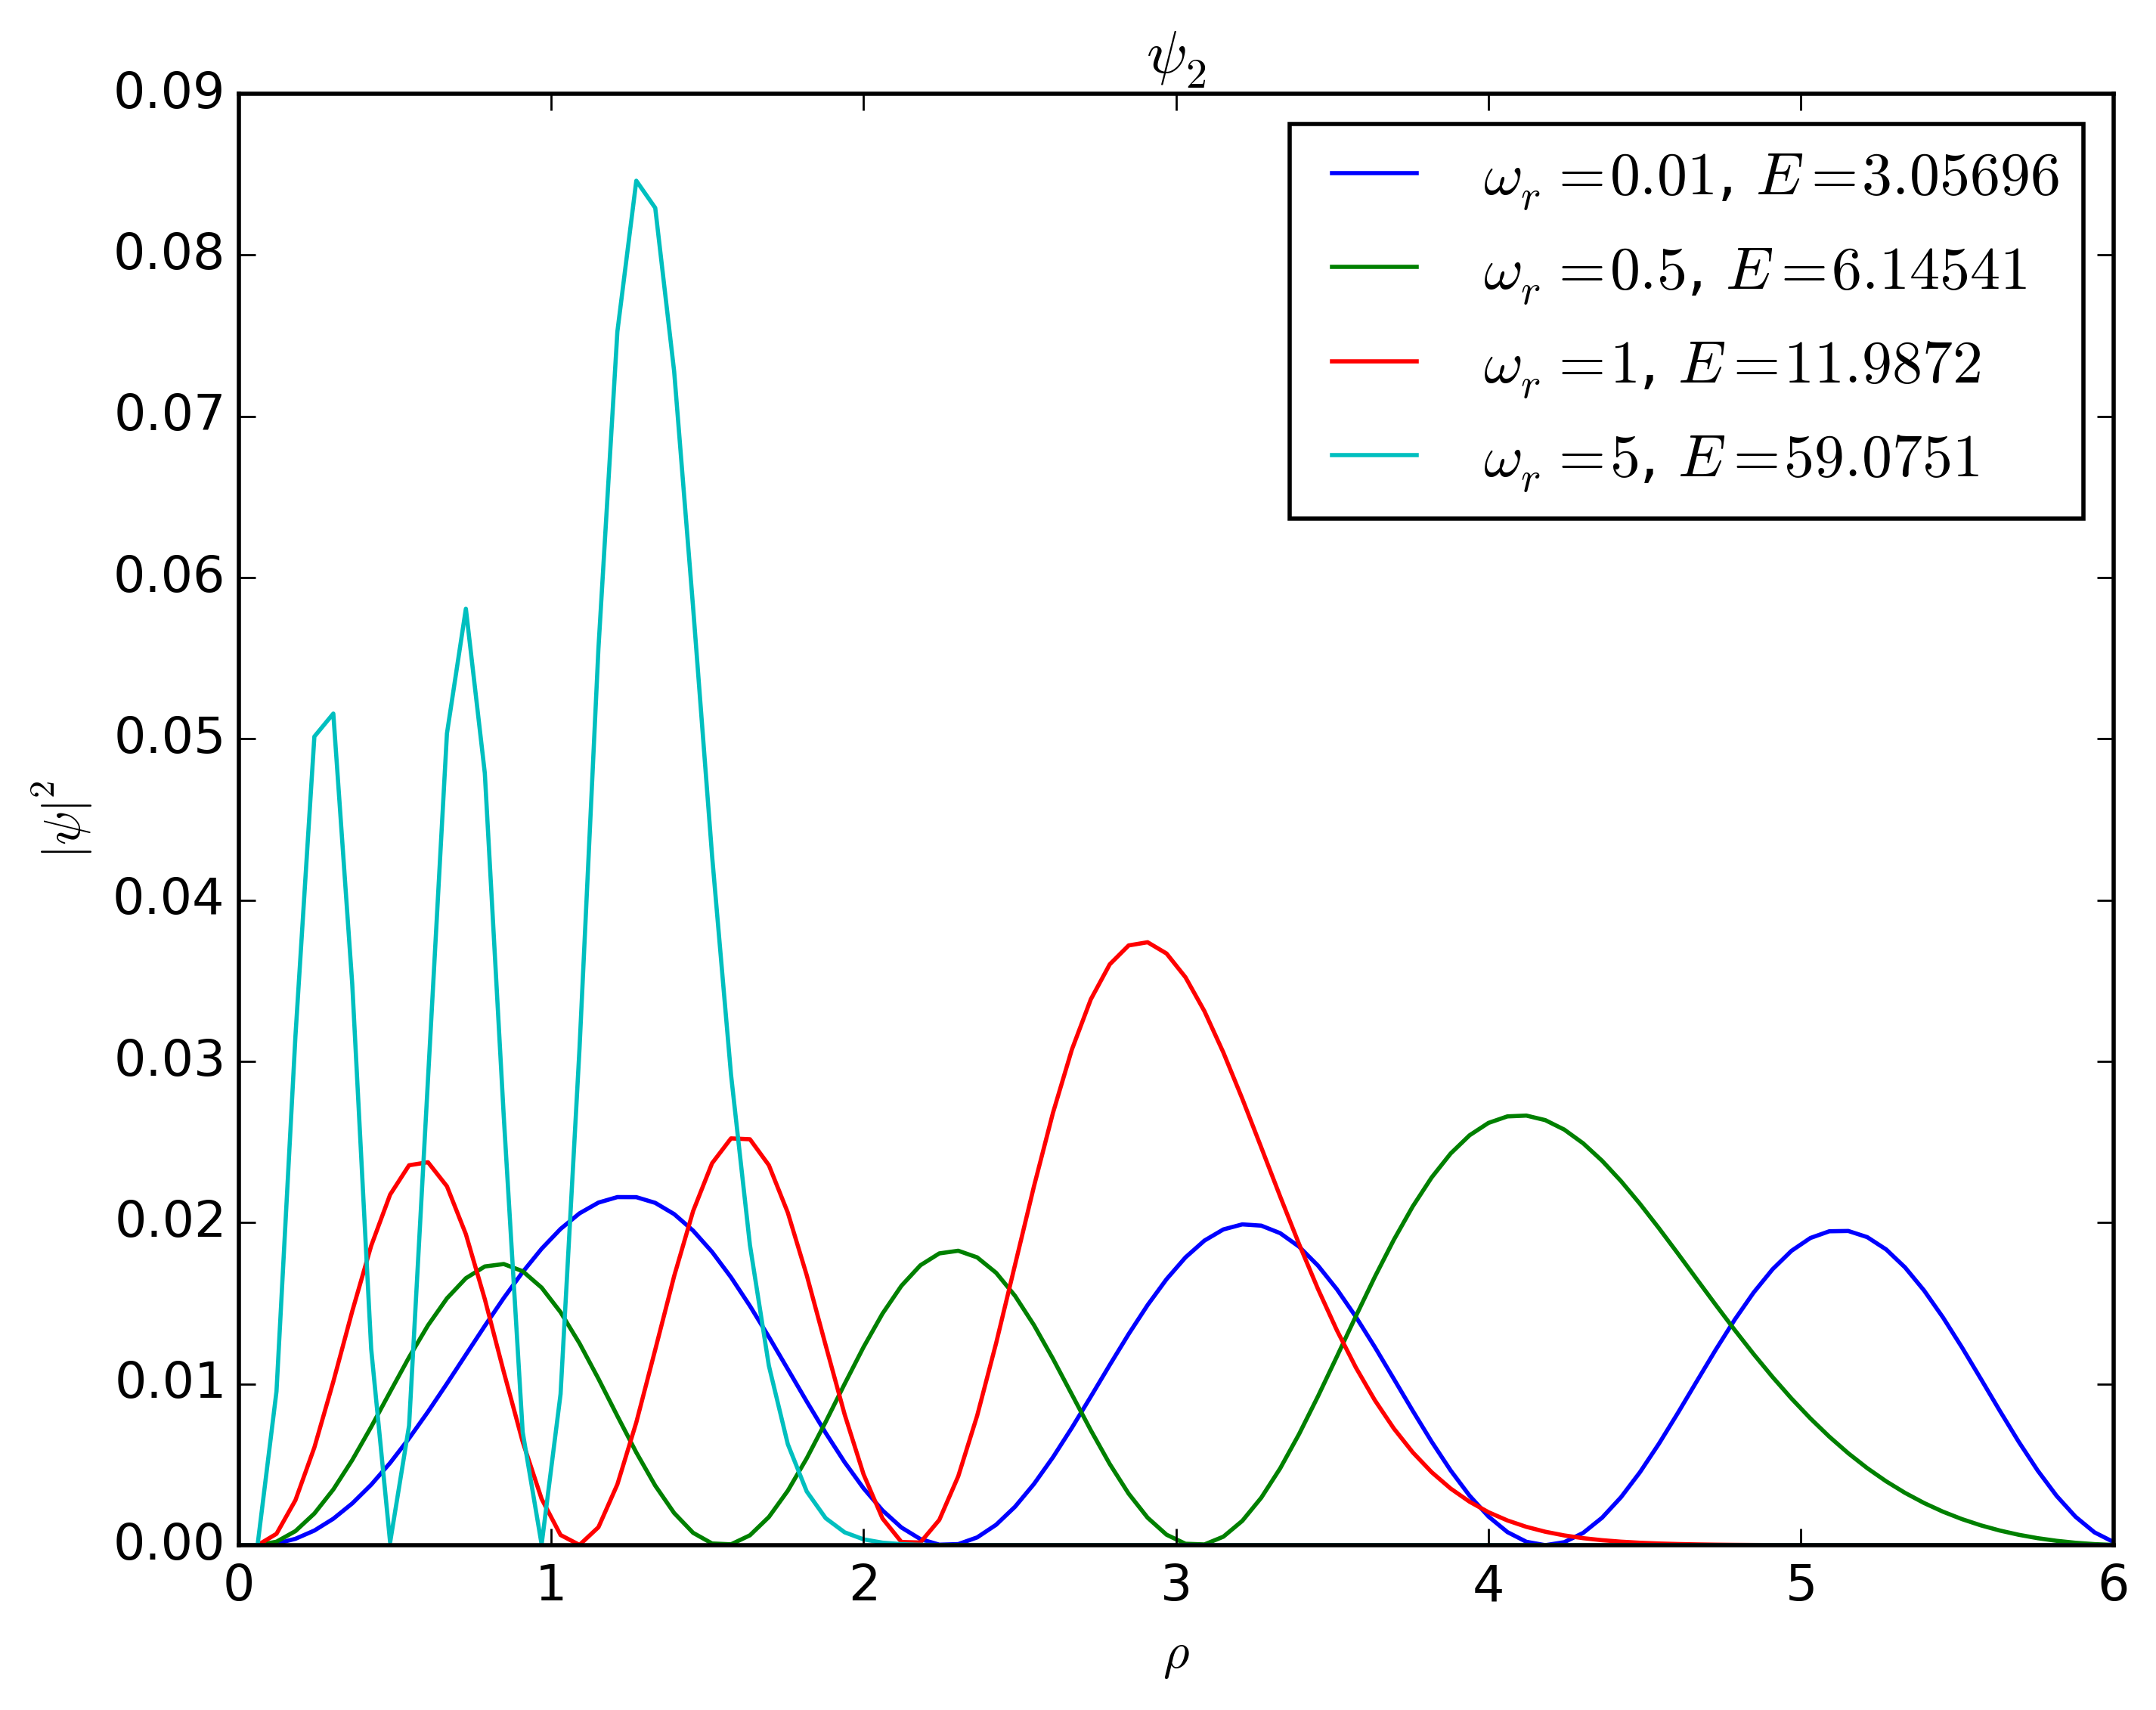
\includegraphics[width=\figurewidth]{../results/psi_compare_omegar2.png}
\caption{Wave function with third lowest energy eigenvalue
for different values of $\omega_r$}
\label{fig:omegar2}
\end{figure}


\section{Concluding remarks }

\end{document}
